% !TEX root = ../main.tex

\chapter{Implementation}
\label{ch:implementation}

\startcontents[chapters]

\vfill

\begin{alltt}\sffamily
Craft against vice I must apply,
you will compel me then to read the will,
this man so complete,
for when thou gav'st them the rod.

A saw a flea stick upon Bardolph's nose,
god may finish it when he will,
deserved thy beauty's use,
you do surely bar the door upon your own liberty.

My heart thy picture's sight would bar,
and finish all foul thoughts,
to dark dishonour's use thou shalt not have.

Their ruth and let me use my sword,
my bare fists I would execute,
is the young Dauphin every way complete.
\end{alltt}

\newpage
\minicontents
\spirals

\begin{figure}[!htbp] % (here, top, bottom, page)
  \centering
  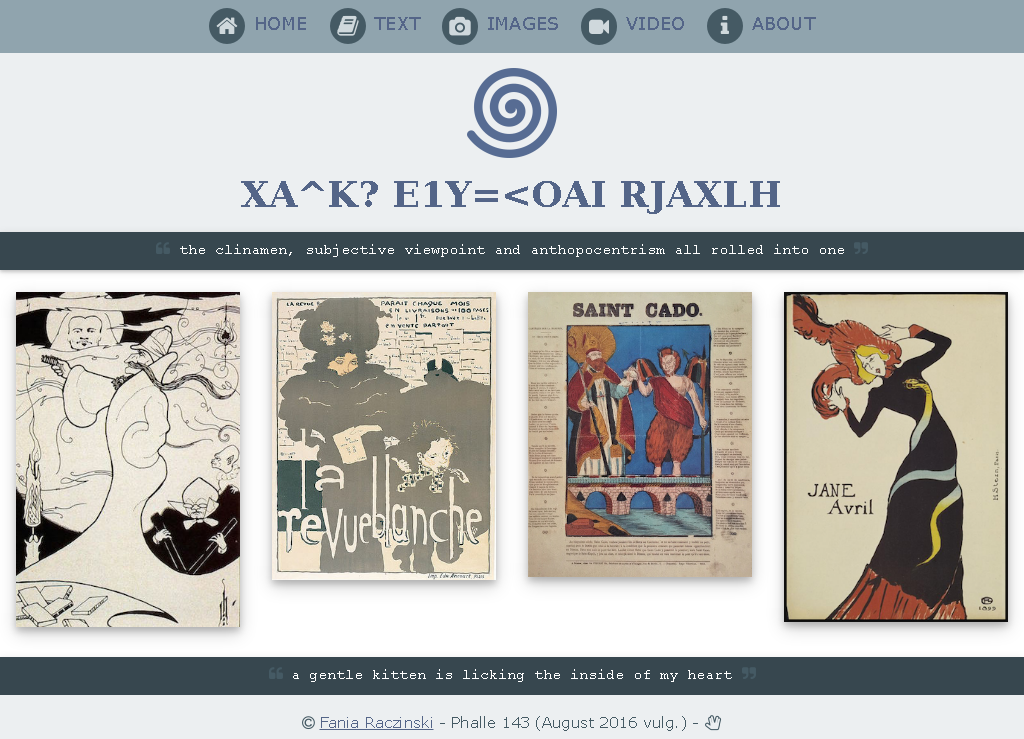
\includegraphics[width=0.95\linewidth]{images/fullscreenshot}
\caption[Screenshot of \url{pata.physics.wtf}]{Screenshot of \url{pata.physics.wtf}\footnotemark}
\label{img:fullscreenshot}
\end{figure}
\footnotetext{The individual letters of the title scramble into place when first loaded. Once this has happend, the title would read: `PATA.PHYSICS.SEARCH'.}

\begin{wrapfigure}{o}{0.4\textwidth}
  \centering
  \scalebox{.8}{
  \begin{forest} folders,
    [pata.physics.wtf, folder
      [app, folder
        [static, folder
          [corpus, folder
            [faustroll, folder]
            [shakespeare, folder]
            [quotes.txt]
          ]
          [css, folder
            [dw\_glidescroll.js]
            [fania.css]
            [fania.js]
            [jquery-1.11.1.min.js]
            [poemscroll.js]
            [scramble.js]
            [tab\_handler.js]
            [w3.css]
          ]
          [images, folder]
        ]
        [templates, folder
          [base.html]
          [header.html]
          [index.html]
          [errors.html]
          [about.html]
          [text.html]
          [textresults.html]
          [images.html]
          [imageresults.html]
          [videos.html]
          [videoresults.html]
        ]
        [\_\_init\_\_.py]
        [views.py]
        [textsurfer.py]
        [textviews.py]
        [imagesurfer.py]
        [imageviews.py]
        [videosurfer.py]
        [videoviews.py]
      ]
      [guni.py]
      [readme.md]
    ]
  \end{forest}
  }
  \caption[Project directory]{Project directory}
  \label{fig:dir}
  \vspace{-2cm}
\end{wrapfigure}

The website \url{http://pata.physics.wtf} (see image~\ref{img:fullscreenshot}\sidepar{\faicon{picture-o}~\ref{img:fullscreenshot}}) embodies the knowledge of this doctoral research and showcases \acf{AMC} and patalgorithms. This chapter gives an overview of the structure of the website and the development process.

A high level view of the site would be that it is a pataphysical search engine that subverts conventional expectations by recombining literary texts into emergent user directed and ephemeral poetical structures or unpredictable spirals of pataphysicalised visual media. 

It is written in 5 different programming languages\footnote{Python, \ac{HTML}, \ac{CSS}, Jinja, JavaScript}, making calls to 6 external web services\footnote{Microsoft Translate, WordNet, Bing, Getty, Flickr and YouTube}, in a total of over \num{3000} lines of code\footnote{\num{2864} lines of code, \num{489} lines of comments - as of 08 Dec 2015} spread over 30 key files. 

Typically, software development is divided into so-called front- and back-ends. The front-end includes web design and web development and is meant to provide an interface for the end-user to communicate with the back-end which involves a server, an application and a database (although this is not fully the case in this project).

The front-end design uses the \textit{W3.CSS} stylesheet \autocite{w3css} as a basis. The website is mostly responsive (see image~\ref{img:proto3screen}\sidepar{\faicon{picture-o}~\ref{img:proto3screen}}), meaning it can be viewed well on phones, tablets and desktop screens (the poems and image spirals for example unfortunately have a fixed width which does not scale down well). The site contains various scripts written in \textbf{JavaScript} (e.g. scramble letters, randomise poem, send email and tabbed content).

The backend relies heavily on a \textbf{Python} \autocite{pythonmain} framework called \textbf{Flask} \autocite{Ronacher2016}. Most of the code is written in Python although some parts require a specific templating language called \textbf{Jinja} \autocite{Jinja2016} which renders content into \ac{HTML}. The application uses several \acs{API}s (Microsoft Translator, Bing, YouTube, Flickr, Getty and WordNet \autocite{TranslatorAPI,BingAPI,YouTubeAPI,FlickrAPI,GettyAPI,Princeton2010,NLTK2016}) and is version controlled using \textbf{Git} \autocite{Git2016}.

The folder structure is shown in figure~\ref{fig:files}\sidepar{\faicon{object-group}~\ref{fig:files}}. Each spot represents one file.

\begin{figure}[!htbp] % (here, top, bottom, page)
  \centering
  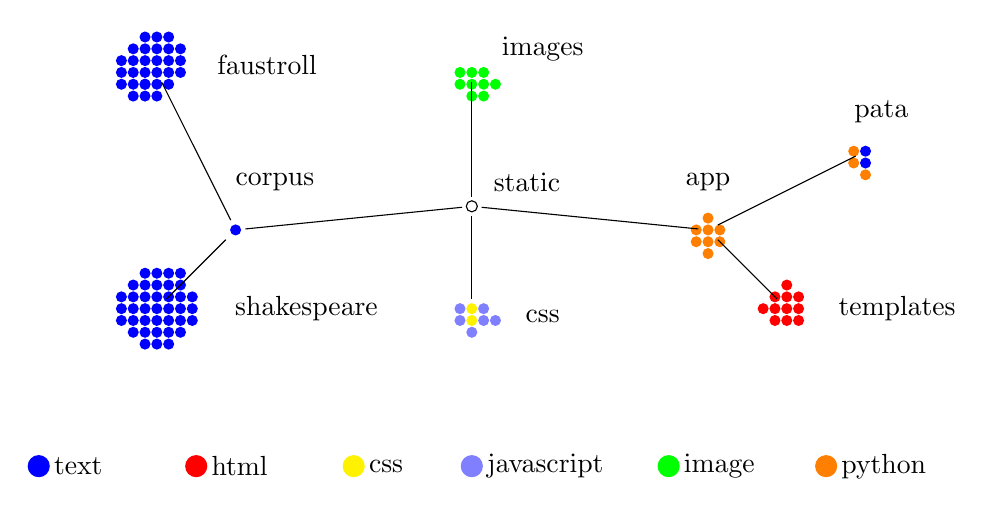
\begin{tikzpicture}
    % \draw[help lines, color=gray] (0,0) grid (13,10);
    \fill [blue] (2,7) circle (2pt) node (faust) {}; % 1
    \fill [blue] (2,7.15) circle (2pt); % 2
    \fill [blue] (2.15,7) circle (2pt); % 3
    \fill [blue] (2.15,7.15) circle (2pt); % 4
    \fill [blue] (2.15,7.3) circle (2pt); % 5
    \fill [blue] (2.3,7.15) circle (2pt); % 6
    \fill [blue] (2.3,7.3) circle (2pt); % 7
    \fill [blue] (1.85,7) circle (2pt); % 8
    \fill [blue] (2,6.85) circle (2pt); % 9
    \fill [blue] (1.85,6.85) circle (2pt); % 10
    \fill [blue] (1.7,6.85) circle (2pt); % 11
    \fill [blue] (1.7,7) circle (2pt); % 12
    \fill [blue] (1.85,7.15) circle (2pt); % 13
    \fill [blue] (1.85,7.3) circle (2pt); % 14
    \fill [blue] (1.85,6.7) circle (2pt); % 15
    \fill [blue] (1.7,6.7) circle (2pt); % 16
    \fill [blue] (2,6.7) circle (2pt); % 17
    \fill [blue] (1.85,6.85) circle (2pt); % 18
    \fill [blue] (2,7.3) circle (2pt); % 19
    \fill [blue] (2.3,7) circle (2pt); % 20
    \fill [blue] (2.15,7.45) circle (2pt); % 21
    \fill [blue] (2.15,6.85) circle (2pt); % 22
    \fill [blue] (1.55,7) circle (2pt); % 23
    \fill [blue] (1.55,6.85) circle (2pt); % 24
    \fill [blue] (1.7,7.15) circle (2pt); % 25
    \fill [blue] (1.7,7.3) circle (2pt); % 26
    \fill [blue] (1.55,7.15) circle (2pt); % 27
    \fill [blue] (2,7.45) circle (2pt); % 28
    \fill [blue] (1.85,7.45) circle (2pt); % 29

    \fill [blue] (2,4) circle (2pt) node (shake) {}; % 1
    \fill [blue] (2,4.15) circle (2pt); % 2
    \fill [blue] (2,4.3) circle (2pt); % 3
    \fill [blue] (2,4.45) circle (2pt); % 4
    \fill [blue] (1.7,4.3) circle (2pt); % 5
    \fill [blue] (2,3.85) circle (2pt); % 6
    \fill [blue] (2,3.7) circle (2pt); % 7
    \fill [blue] (2,3.55) circle (2pt); % 8
    \fill [blue] (1.85,4) circle (2pt); % 9
    \fill [blue] (1.7,4) circle (2pt); % 10
    \fill [blue] (1.55,4) circle (2pt); % 11
    \fill [blue] (2.15,3.7) circle (2pt); % 12
    \fill [blue] (2.15,4) circle (2pt); % 13
    \fill [blue] (2.3,4) circle (2pt); % 14
    \fill [blue] (2.45,4) circle (2pt); % 15
    \fill [blue] (2.45,3.85) circle (2pt); % 16
    \fill [blue] (2.3,3.85) circle (2pt); % 17
    \fill [blue] (2.15,3.55) circle (2pt); % 18
    \fill [blue] (2.15,4.15) circle (2pt); % 19
    \fill [blue] (2.3,4.15) circle (2pt); % 20
    \fill [blue] (2.3,4.3) circle (2pt); % 21
    \fill [blue] (2.3,4.45) circle (2pt); % 22
    \fill [blue] (2.45,4.15) circle (2pt); % 23
    \fill [blue] (2.3,3.7) circle (2pt); % 24
    \fill [blue] (2.15,4.3) circle (2pt); % 25
    \fill [blue] (2.15,4.45) circle (2pt); % 26
    \fill [blue] (1.85,4.15) circle (2pt); % 27
    \fill [blue] (1.85,4.3) circle (2pt); % 28
    \fill [blue] (1.85,4.45) circle (2pt); % 29
    \fill [blue] (1.7,4.15) circle (2pt); % 30
    \fill [blue] (1.55,4.15) circle (2pt); % 31
    \fill [blue] (1.85,3.85) circle (2pt); % 32
    \fill [blue] (1.85,3.7) circle (2pt); % 33
    \fill [blue] (1.85,3.55) circle (2pt); % 34
    \fill [blue] (1.7,3.85) circle (2pt); % 35
    \fill [blue] (1.7,3.7) circle (2pt); % 36
    \fill [blue] (1.55,3.85) circle (2pt); % 37
    \fill [blue] (2.15,3.85) circle (2pt); % 38
    
    \fill [yellow] (6,4) circle (2pt) node (css) {}; % 1
    \fill [yellow] (6,3.85) circle (2pt); % 2
    \fill [blue!50!white] (6,3.7) circle (2pt); % 3
    \fill [blue!50!white] (5.85,3.85) circle (2pt); % 4
    \fill [blue!50!white] (5.85,4) circle (2pt); % 5
    \fill [blue!50!white] (6.15,3.85) circle (2pt); % 6
    \fill [blue!50!white] (6.15,4) circle (2pt); % 7
    \fill [blue!50!white] (6.3,3.85) circle (2pt); % 8
    
    \fill [green] (6,7) circle (2pt) node (imgs) {}; % 1
    \fill [green] (6,6.85) circle (2pt); % 2
    \fill [green] (6,6.7) circle (2pt); % 3
    \fill [green] (5.85,6.85) circle (2pt); % 4
    \fill [green] (5.85,7) circle (2pt); % 5
    \fill [green] (6.15,6.85) circle (2pt); % 6
    \fill [green] (6.15,7) circle (2pt); % 7
    \fill [green] (6.3,6.85) circle (2pt); % 8
    \fill [green] (6.15,6.7) circle (2pt); % 9
    
    \fill [blue] (3,5) circle (2pt) node (corpus) {};
    \draw (6,5.3) circle (2pt) node (static) {};
    
    \fill [red] (10,4) circle (2pt) node (temp) {}; % 1
    \fill [red] (10,4.15) circle (2pt); % 2
    \fill [red] (10,4.3) circle (2pt); % 3
    \fill [red] (10.15,4.15) circle (2pt); % 4
    \fill [red] (9.85,4.15) circle (2pt); % 5
    \fill [red] (10,3.85) circle (2pt); % 6
    \fill [red] (10.15,3.85) circle (2pt); % 7
    \fill [red] (10.15,4) circle (2pt); % 8
    \fill [red] (9.85,4) circle (2pt); % 9
    \fill [red] (9.7,4) circle (2pt); % 10
    \fill [red] (9.85,3.85) circle (2pt); % 11
    
    \fill [orange] (9,5) circle (2pt) node (app) {}; % 1
    \fill [orange] (9,4.85) circle (2pt); % 2
    \fill [orange] (9,4.7) circle (2pt); % 3
    \fill [orange] (8.85,4.85) circle (2pt); % 4
    \fill [orange] (8.85,5) circle (2pt); % 5
    \fill [orange] (9.15,4.85) circle (2pt); % 6
    \fill [orange] (9.15,5) circle (2pt); % 7
    \fill [orange] (9,5.15) circle (2pt); % 8
      
    \fill [blue] (11,6) circle (2pt) node (main) {}; % 1
    \fill [blue] (11,5.85) circle (2pt); % 2
    \fill [orange] (11,5.7) circle (2pt); % 3
    \fill [orange] (10.85,5.85) circle (2pt); % 4
    \fill [orange] (10.85,6) circle (2pt); % 5
    
    \draw (faust) -- (corpus);
    \node at (3.4,7.1) {faustroll};
    \draw (shake) -- (corpus);
    \node at (3.9,4) {shakespeare};
    \draw (corpus) -- (static);
    \node at (3.5,5.6) {corpus};
    \draw (imgs) -- (static);
    \node at (6.9,7.3) {images};
    \draw (css) --(static);
    \node at (6.9,3.9) {css};
    \draw (static) -- (app);
    \node at (6.7,5.6) {static};
    \draw (temp) -- (app);
    \node at (11.4,4) {templates};
    \draw (app) -- (main);
    \node at (9,5.6) {app};
    \node at (11.2,6.5) {pata};
    
    \fill [blue] (0.5,2) circle (4pt) node [right=2pt, black] (txt) {text};
    \fill [green] (8.5,2) circle (4pt) node [right=2pt, black] (img) {image};
    \fill [orange] (10.5,2) circle (4pt) node [right=2pt, black] (py) {python};
    \fill [red] (2.5,2) circle (4pt) node [right=2pt, black] (html) {html};
    \fill [yellow] (4.5,2) circle (4pt) node [right=2pt, black] (css) {css};
    \fill [blue!50!white] (6,2) circle (4pt) node [right=2pt, black] (js) {javascript};
  \end{tikzpicture}
\caption[Folder structure and file types]{Folder structure and file types}
\label{fig:files}
\end{figure}

Figures~\ref{fig:textsearch} and~\ref{fig:visualsearch} show the two main workflow scenarios of \url{pata.physics.wtf} in the form of sequence diagrams. The columns are labeled with the main agents (this includes the user and the various main files responsible for key actions in the system). Going down vertically represents time. 

Figure~\ref{fig:textsearch}\sidepar{\faicon{object-group}~\ref{fig:textsearch}} demonstrates an outline of how the text search process works. A user enters a query into a search box in the \py{text.html} file which is rendered by the \py{textviews.py} file. Then it gets forwarded to the \py{textsurfer.py} file which then handles the pataphysicalisation process and returns patadata back to \py{textviews.py}. This python file then passes it on to the \py{textresults.html} file which retrieves and renders the results to the user. The user then has the option to randomise the results (if displayed as a poem) which is handled by the \py{fania.js} file. A very similar process is in place for image and video search as shown in figure~~\ref{fig:visualsearch}\sidepar{\faicon{object-group}~\ref{fig:visualsearch}}. The main difference is the results are retrieved in the \py{fania.js} file rather than the \py{imgresults.html} file.

\begin{figure}[!p] % (here, top, bottom, page)
  \centering
  \begin{minipage}[c]{\textwidth}
    \begin{tikzpicture}[every node/.style={font=\normalsize,
      minimum height=0.5cm,minimum width=0.5cm},]

    % Matrix
    \node [matrix, very thin,column sep=2cm,row sep=0.5cm] (matrix) at (0,0) {
      % files
      \node(user){}; &[-0.8cm] \node(th){}; &[-0.1cm] \node(tvp){}; &[0.3cm] \node(tsp){}; &[0.6cm] \node(trh){}; &[0.2cm] \node(fj){}; \\
      % row 1
      \node(user 1){}; & \node(th 1){}; & \node(tvp 1){}; & \node(tsp 1){}; & & \\
      % horizontal line 1
      \node(t1 left){}; & & & & & \node(t1 right){};\\
      % row 2
      & & \node(tvp 2){}; & \node(tsp 2){}; & & \\
      % horizontal line 2
      \node(t2 left){}; & & & & & \node(t2 right){};\\
      % row 3
      & & \node(tvp 3){}; & \node(tsp 3){}; & \node(trh 3){}; & \node(fj 3){};\\
      % horizontal line 3
      \node(t3 left){}; & & & & & \node(t3 right){};\\
      % row 4
      \node(user 4){}; & \node(th 4){}; & \node(tvp 4){}; & \node(tsp 4){}; & \node(trh 4){}; & \node(fj 4){};\\
      % horizontal line 4
      \node(t4 left){}; & & & & & \node(t4 right){};\\
      % row 5
      \node(user 5){}; & \node(th 5){}; & \node(tvp 5){}; & \node(tsp 5){}; & \node(trh 5){}; & \node(fj 5){};\\
      % horizontal line 5
      \node(t5 left){}; & & & & & \node(t5 right){};\\
      % row 6
      \node(user 6){}; & \node(th 6){}; & \node(tvp 6){}; & \node(tsp 6){}; & \node(trh 6){}; & \node(fj 6){};\\
      % last row
      \node(user 7){}; & \node(th 7){}; & \node(tvp 7){}; & \node(tsp 7){}; & \node(trh 7){}; & \node(fj 7){};\\
    };

    % Files
    \fill 
      (user) node[draw,fill=white] {User}
      (th) node[draw,fill=white] {text.html}
      (tvp) node[draw,fill=white] {textviews.py}
      (tsp) node[draw,fill=white] {textsurfer.py}
      (trh) node[draw,fill=white] {textresults.html}
      (fj) node[draw,fill=white] {fania.js};

    % Horizontal lines
    \draw [dotted] 
      (t1 left) -- (t1 right)
      (t2 left) -- (t2 right)
      (t3 left) -- (t3 right)
      (t4 left) -- (t4 right)
      (t5 left) -- (t5 right);

    % Vertical lines
    \draw [dashed] 
      (user) -- (user 7)
      (th) -- (th 7)
      (tvp) -- (tvp 7)
      (tsp) -- (tsp 7)
      (trh) -- (trh 7)
      (fj) -- (fj 7);

    % Blocks
    \filldraw[fill=white]
      (user 1.north west) rectangle (user 6.south east)
      (th 1.north west) rectangle (th 1.south east)
      (tvp 1.north west) rectangle (tvp 3.south east)
      (tsp 1.north west) rectangle (tsp 2.south east)
      (trh 3.north west) rectangle (trh 4.south east)
      (trh 5.north west) rectangle (trh 6.south east)
      (fj 5.north west) rectangle (fj 6.south east);

    % Horizontal flows
    \draw [arr] (user 1) -- node[txt]{query} (th 1);
    \draw [arr] (th 1) -- node[txt]{query} (tvp 1);
    \draw [arr] (tvp 1) -- node[txt]{query} (tsp 1);
    \draw [arr] (tsp 2) -- node[txt]{patadata} (tvp 2);
    \draw [arr] (tvp 3) -- node[txt]{results} (tsp 3.west) arc(180:0:0.25cm) -- (trh 3);
    \draw [arr] (trh 4) -- node[txt]{results} (tsp 4.east) arc(0:180:0.25cm) -- (tvp 4.east) arc(0:180:0.25cm) -- (th 4.east) arc(0:180:0.25cm) -- (user 4);

    \draw [arr] (user 5) -- (th 5.west) arc(180:0:0.25cm) -- (tvp 5.west) arc(180:0:0.25cm) -- (tsp 5.west) arc(180:0:0.25cm) -- node[txt]{randomise} (trh 5);
    \draw [arr] (trh 5) -- node[txt]{randomise} (fj 5);
    \draw [arr] (fj 6) -- node[txt]{results} (trh 6);
    \draw [arr] (trh 6) -- node[txt]{results} (tsp 6.east) arc(0:180:0.25cm) -- (tvp 6.east) arc(0:180:0.25cm) -- (th 6.east) arc(0:180:0.25cm) -- (user 6);
    \end{tikzpicture}
    \vspace{-1cm}
    \captionof{figure}{Top-level overview of text search}
    \label{fig:textsearch}
  \end{minipage}%
  % \vspace{0.5\textheight}
  % \vfill%
  \vspace{2cm}
  \begin{minipage}[c]{\textwidth}
    \begin{tikzpicture}[every node/.style={font=\normalsize,
      minimum height=0.5cm,minimum width=0.5cm},]

    % Matrix
    \node [matrix, very thin,column sep=2cm,row sep=0.5cm] (matrix) at (0,0) {
      % files
      \node(user){}; &[-0.6cm] \node(th){}; &[0.15cm] \node(tvp){}; &[0.35cm] \node(tsp){}; &[0.7cm] \node(trh){}; &[0.2cm] \node(fj){}; \\
      % row 1
      \node(user 1){}; & \node(th 1){}; & \node(tvp 1){}; & \node(tsp 1){}; & & \\
      % horizontal line 1
      \node(t1 left){}; & & & & & \node(t1 right){};\\
      % row 2
      & & \node(tvp 2){}; & \node(tsp 2){}; & & \\
      % horizontal line 2
      \node(t2 left){}; & & & & & \node(t2 right){};\\
      % row 3
      & & \node(tvp 3){}; & \node(tsp 3){}; & \node(trh 3){}; & \node(fj 3){};\\
      % horizontal line 3
      \node(t3 left){}; & & & & & \node(t3 right){};\\
      % row 4
      \node(user 4){}; & \node(th 4){}; & \node(tvp 4){}; & \node(tsp 4){}; & \node(trh 4){}; & \node(fj 4){};\\
      % last row
      \node(user 7){}; & \node(th 7){}; & \node(tvp 7){}; & \node(tsp 7){}; & \node(trh 7){}; & \node(fj 7){};\\
    };

    % Files
    \fill 
      (user) node[draw,fill=white] {User}
      (th) node[draw,fill=white] {image.html}
      (tvp) node[draw,fill=white] {imgviews.py}
      (tsp) node[draw,fill=white] {imgsurfer.py}
        (trh) node[draw,fill=white] {imgresults.html}
        (fj) node[draw,fill=white] {fania.js};

    % Horizontal lines
    \draw [dotted] 
      (t1 left) -- (t1 right)
      (t2 left) -- (t2 right)
      (t3 left) -- (t3 right)
      (t4 left) -- (t4 right);

    % Vertical lines
    \draw [dashed] 
      (user) -- (user 7)
      (th) -- (th 7)
      (tvp) -- (tvp 7)
      (tsp) -- (tsp 7)
      (trh) -- (trh 7)
      (fj) -- (fj 7);

    % Blocks
    \filldraw[fill=white]
      (user 1.north west) rectangle (user 4.south east)
      (th 1.north west) rectangle (th 1.south east)
      (tvp 1.north west) rectangle (tvp 3.south east)
      (tsp 1.north west) rectangle (tsp 2.south east)
      (trh 3.north west) rectangle (trh 4.south east)
      (fj 3.north west) rectangle (fj 4.south east);

    % Horizontal flows
    \draw [arr] (user 1) -- node[txt]{query} (th 1);
    \draw [arr] (th 1) -- node[txt]{query} (tvp 1);
    \draw [arr] (tvp 1) -- node[txt]{query} (tsp 1);
    \draw [arr] (tsp 2) -- node[txt]{patadata} (tvp 2);
    \draw [arr] (tvp 3) -- node[txt]{patadata} (tsp 3.west) arc(180:0:0.25cm) -- (trh 3);
    \draw [arr] (trh 3) -- node[txt]{patadata} (fj 3);
    \draw [arr] (fj 4) -- node[txt]{results} (trh 4);
    \draw [arr] (trh 4) -- node[txt]{results} (tsp 4.east) arc(0:180:0.25cm) -- (tvp 4.east) arc(0:180:0.25cm) -- (th 4.east) arc(0:180:0.25cm) -- (user 4);
    \end{tikzpicture}
    \vspace{-1cm}
    \captionof{figure}{Top-level overview of image / video search}
    \label{fig:visualsearch}
  \end{minipage}
\end{figure}
	
% \begin{tikzpicture}[every node/.style={font=\normalsize,
%       minimum height=0.5cm,minimum width=0.5cm},]
%   % Matrix
%   \node [matrix, very thin,column sep=2cm,row sep=0.5cm] (matrix) at (0,0) {
%   % files
%   \node(pata){}; & \node(setup){}; & \node(corpus){};\\
%   % row 1
%   \node(pata 1){}; & \node(setup 1){}; & \node(corpus 1){};\\
%   % horizontal line 1
%   \node(t1 left){}; & & \node(t1 right){};\\
%   % row 2
%   \node(pata 2){}; & \node(setup 2){}; & \node(corpus 2){};\\
%   % horizontal line 2
%   \node(t2 left){}; & & \node(t2 right){};\\
%   % row 3
%   \node(pata 3){}; & \node(setup 3){}; & \node(corpus 3){};\\
%   % last row
%   \node(pata 7){}; & \node(setup 7){}; & \node(corpus 7){};\\
%   };

%   % Files
%   \fill 
%     (pata) node[draw,fill=white] {Pata}
%     (setup) node[draw,fill=white] {Setup}
%     (corpus) node[draw,fill=white] {Corpus};

%   % Horizontal lines
%   \draw [dotted] 
%     (t1 left) -- (t1 right)
%     (t2 left) -- (t2 right);

%   % Vertical lines
%   \draw [dashed] 
%     (pata) -- (pata 7)
%     (setup) -- (setup 7)
%     (corpus) -- (corpus 7);

%   % Blocks
%   \filldraw[fill=white]
%     (pata 1.north west) rectangle (pata 3.south east)
%     (setup 1.north west) rectangle (setup 2.south east)
%     (setup 3.north west) rectangle (setup 3.south east)
%     (corpus 1.north west) rectangle (corpus 2.south east);

%   % Horizontal flows
%   \draw [arr] (pata 1) -- node[txt]{load} (setup 1);
  
%   \draw [arr] (setup 1) -- node[txt]{open file} (corpus 1);
%   \draw [arr] (corpus 2) -- node[txt]{read text} (setup 2);
%   \draw [arr] (setup 2) -- node[txt,right,fill=white]{add to index} (setup 3);
%   \draw (2.7,1) node[txt,fill=white]{loop};
%   \draw (-0.6,0.9) rectangle (3.2,6); % loop
%   \draw [arr] (setup 3) -- node[txt]{} (pata 3);
%   \end{tikzpicture}

Putting it another way, (1) the system setup tokenises each of the source texts, removes stopwords and then adds terms and their location to the index (see section~\ref{s:index}\sidepar{§~\ref{s:index}}), (2) a query then triggers the three pataphysical algorithms, (3) each algorithm finds results for the query (see section~\ref{s:algorithms}\sidepar{§~\ref{s:algorithms}}), (4) some words before/after the match are retrieved for context, and (5) the resulting sentences are rendered for the user.

\spirals

The following sections discuss the initial setup of the system when it is first started up, the text search algorithms, the image and video \ac{API} calls and the main design elements (text poetry and image spirals).


\section{Setup}
\label{s:setup}

The Python web framework Flask \autocite{Ronacher2016} looks after loading and rendering the various pages for \url{pata.physics.wtf} (home, text-search, text-results, image-search, image-results, video-search, video-results, about and errors), which means most of the backend related code is written in Python. Although Flask contains a small development server, in a production environment a more capable server is needed. For this reason the Flask site runs on a Gunicorn server \autocite{Gunicorn2016} and is hosted on a UNIX machine.


\subsection{Corpora}
\label{s:corpora}

Instead of crawling the Internet \url{pata.physics.wtf} uses a local collection of texts for its text search. Setting up a custom web crawler would require a lot more resources (in terms of hardware, time and money) than practical for this project. There are two corpora containing 65 text files together. 

The first corpus resembles the fictional library of `equivalent books' from Jarry's \textit{Exploits and Opinions of Dr.\ Faustroll, $'$Pataphysician} \autocite*{Jarry1996}. In principle the corpus is just a folder within the tool's directory structure containing the following files:

% \footnote{`In addition, three prints hanging on the walls, a poster by TOULOUSE-LAUTREC, \emph{Jane Avril}; one by BONNARD, advertising the \emph{Revue Blanche}; a portrait of Doctor Faustroll, by AUBREY BEARDSLEY\@; and an old picture, which appeared to us to be valueless, \emph{Saint Cado}, issued by the Oberthuer printing house of Rennes.'\parencite[p.12]{Jarry1996}}

\begin{enumerate}[start=0]
\item Alfred Jarry: \textit{Exploits and Opinions of Dr.\ Faustroll, $'$Pataphysician} \autocite*{Jarry1996}
\item Edgar Allen Poe: \textit{Collected Works} \autocite*{Poe2008}
\item Cyrano de Bergerac: \textit{A Voyage to the Moon} \autocite*{Bergerac2014}
\item Saint Luke: \textit{The Gospel} \autocite*{Bergerac2014}
\item L{\'e}on Bloy: \textit{Le D{\'e}sesp{\'e}r{\'e}} (French) \autocite*{Bloy2011}
\item Samuel Taylor Coleridge: \textit{The Rime of the Ancient Mariner} \autocite*{Coleridge2013}
\item Georges Darien: \textit{Le Voleur} (French) \autocite*{Darien2005}
\item Marceline Desbordes-Valmore: \textit{Le Livre des M{\`e}res et des Enfants} (French) \autocite*{Desbordes2004}
\item Max Elskamp: \textit{Enluminures} (French) \autocite*{Elskamp1898}
\item Jean-Pierre Claris de Florian: \textit{Les Deux Billets} (French) \autocite*{Florian2012}
\item \textit{One Thousand and One Nights} \autocite{Lang2008}
\item Christian Grabbe: \textit{Scherz, Satire, Ironie und tiefere Bedeutung} (German) \autocite*{Grabbe1995}
\item Gustave Kahn: \textit{Le Conte de l'Or et Du Silence} (French) \autocite*{Kahn2016}
\item Le Comte de Lautr{\'e}amont: \textit{Les Chants de Maldoror} (French) \autocite*{Lautreamont2011}
\item Maurice Maeterlinck: \textit{Aglavaine and S{\'e}lysette} \autocite*{Maeterlinck1918}
\item St{\'e}phane Mallarm{\'e}: \textit{Verse and Prose} (French) \autocite*{Mallarme2003}
\item Catulle Mend{\`e}s: \textit{The Mirror} and \textit{la Divina Aventure} (English and Spanish) \autocite*{Mendes1910,Mendes2013}
\item Homer: \textit{The Odyssey} \autocite*{Homer1999}
\item Jos{\'e}phin P{\'e}ladan: \textit{Babylon} (EMPTY FILE)\footnote{I have not been able to find any source texts online.\label{emptyfile}}
\item Fran\c{c}ois Rabelais: \textit{Gargantua and Pantagruel} \autocite*{Rabelais2004}
\item Jean de Chilra: \textit{L'Heure Sexuelle} (EMPTY FILE)\textsuperscript{\ref{emptyfile}}
\item Henri de R{\'e}gnier: \textit{La Canne de Jaspe} (EMPTY FILE)\textsuperscript{\ref{emptyfile}}
\item Arthur Rimbaud: \textit{Poesies Completes} (French) \autocite*{Rimbaud2009}
\item Marcel Schwob: \textit{Der Kinderkreuzzug} (German) \autocite*{Schwob2012}
\item Alfred Jarry: \textit{Ubu Roi} (French) \autocite*{Jarry2005}
\item Paul Verlaine: \textit{Poems} \autocite*{Verlaine2009}
\item Emile Verhaeren: \textit{Poems} \autocite*{Verhaeren2010}
\item Jules Verne: \textit{A Journey to the Centre of the Earth} \autocite*{Verne2010}
\end{enumerate}

The original list as it appears in `Faustroll' is shown in chapter~\ref{s:faustlib}\sidepar{§~\ref{s:faustlib}}. Three of the items have not been found as a resource. Some others have been approximated by using another text by the same author for example. Most of these were sourced from \emph{Project Gutenberg} \autocite{Gutenberg2016} in their original languages. The decision to get foreign language texts was partially due to the lack of out-of-copyright translated versions and partially because the original library in `Faustroll' was also multi-lingual.

\textbf{A note on copyright:} UK copyright law states in section 5 that the duration of copyright for ``literary, dramatic, musical or artistic works'' is ``70 years from the end of the calendar year in which the last remaining author of the work dies'' \autocite{Copyright2015}. Maurice Maeterlinck and Marguerite Vallette-Eymery (a.k.a. Rachilde or Jean de Chilra) died less than 70 years ago and their work should still be under copyright. Alfred Jarry in the Simon Watson Taylor translation is a derivative work and is probably also still protected. However, copyright does not apply when used for ``private and research study purposes'' as stated in section 7 on \textit{Fair dealing} of \autocite{Copyright2012}.

The second corpus is a collection of 38 texts by William Shakespeare \autocite*{Shakespeare2011}.

\begin{enumerate}
  \item \textit{The Sonnets}
  \item \textit{Alls Well That Ends Well}
  \item \textit{The Tragedy of Antony and Cleopatra}
  \item \textit{As You Like It}
  \item \textit{The Comedy of Errors}
  \item \textit{The Tragedy of Coriolanus}
  \item \textit{Cymbeline}
  \item \textit{The Tragedy of Hamlet, Prince of Denmark}
  \item \textit{The First Part of King Henry the Fourth}
  \item \textit{The Second Part of King Henry the Fourth}
  \item \textit{The Life of Kind Henry the Fifth}
  \item \textit{The First Part of Henry the Sixth}
  \item \textit{The Second Part of Henry the Sixth}
  \item \textit{The Third Part of Henry the Sixth}
  \item \textit{King Henry the Eigth}
  \item \textit{King John}
  \item \textit{The Tragedy of Julius Caesar}
  \item \textit{The Tragedy of King Lear}
  \item \textit{Love's Labour's Lost}
  \item \textit{The Tragedy of Macbeth}
  \item \textit{Measure for Measure}
  \item \textit{The Merchant of Venice}
  \item \textit{The Merry Wives of Windsor}
  \item \textit{A Midsummer Night's Dream}
  \item \textit{Much Ado About Nothing}
  \item \textit{The Tragedy of Othello, Moor of Venice}
  \item \textit{King Richard the Second}
  \item \textit{Kind Richard III}
  \item \textit{The Tragedy of Romeo and Juliet}
  \item \textit{The Taming of the Shrew}
  \item \textit{The Tempest}
  \item \textit{The Life of Timon of Athens}
  \item \textit{The Tragedy of Titus Andronicus}
  \item \textit{The History of Troilus and Cressida}
  \item \textit{Twelfth Night or What You Will}
  \item \textit{The Two Gentlemen of Verona}
  \item \textit{The Winter's Tale}
  \item \textit{A Lover's Complaint}
\end{enumerate}

% \begin{figure}[!htbp]
% \centering
% \begin{minipage}{.45\linewidth}
%   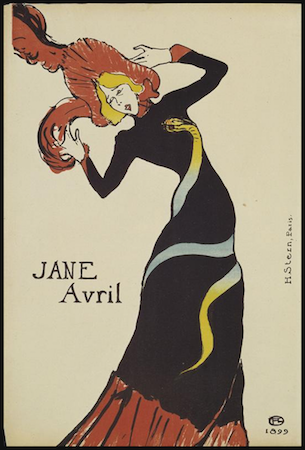
\includegraphics[width=\linewidth]{JaneAvril}
%   \caption[Toulouse-Lautrec's ``Jane Avril'']{Toulouse-Lautrec's ``Jane Avril''}
% \label{fig:toulouse}
% \end{minipage}
% \hspace{.05\linewidth}
% \begin{minipage}{.45\linewidth}
%   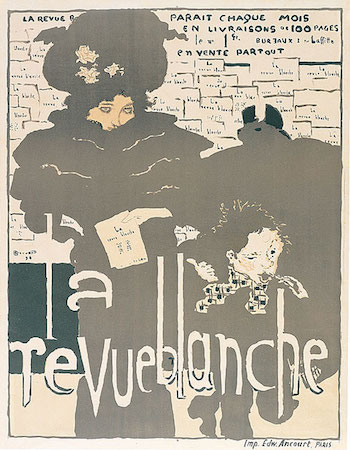
\includegraphics[width=\linewidth]{RevueBlanche}
%   \caption[Bonnard's ``Revue Blanche'']{Bonnard's ``Revue Blanche''}
% \label{fig:bonnard}
% \end{minipage}
% \vspace{.05\linewidth}
% \begin{minipage}{.45\linewidth}
%   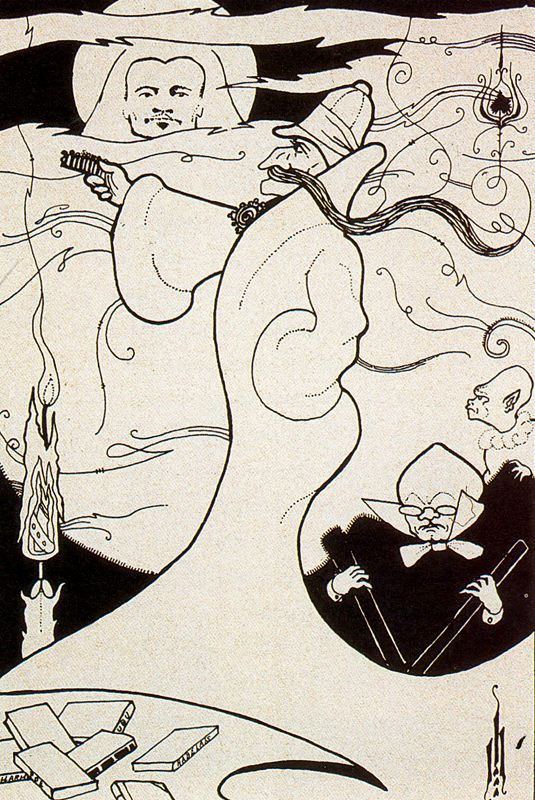
\includegraphics[width=\linewidth]{DocteurFaustroll}
%   \caption[Aubrey Beardsley's ``Docteur Faustroll'']{Aubrey Beardsley's ``Docteur Faustroll''}
% \label{fig:beardsley}
% \end{minipage}
% \hspace{.05\linewidth}
% \begin{minipage}{.45\linewidth}
%   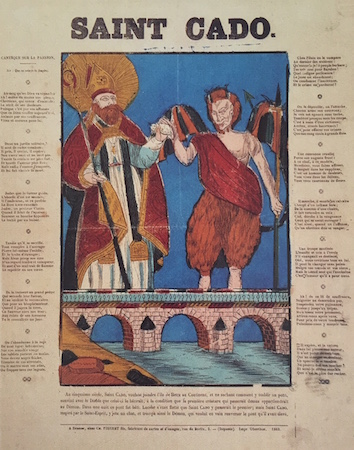
\includegraphics[width=\linewidth]{SaintCado}
%   \caption[Oberthuer's ``Saint Cado'']{Oberthuer's ``Saint Cado''}
% \label{fig:oberthuer}
% \end{minipage}
% \end{figure}


\subsection{Index}
\label{s:index}

When the server is first started various setup functions (such as the creation of the index) are executed before any \ac{HTML} is rendered. The search algorithms are triggered once a user enters a search term into the query field on any of the text, image or video pages.

Each plain text file in the corpus is added to the internal library one by one. Source~\ref{code:addtocorpus}\sidepar{\faicon{code}~\ref{code:addtocorpus}} shows how this is done. The \py{PlaintextCorpusReader} is a feature of the \ac{NLTK} Python library \autocite{NLTK2016} for \acf{NLP}. The \py{words} function tokenises the text, i.e. it splits it into individual words and stores them as an ordered list.

\begin{listing}[!htbp] % (here, top, bottom, page)
  \begin{minted}{python}
library = PlaintextCorpusReader(corpus_root, '.*\.txt')
l_00 = library.words('00.faustroll.txt')
l_01 = library.words('01.poe1.txt')
...
l_27 = library.words('27.verne.txt')
  \end{minted}
\caption{Adding text files to the corpus library}
\label{code:addtocorpus}
\end{listing}

The \py{setupcorpus} function (see source~\ref{code:setupcorpus}\sidepar{\faicon{code}~\ref{code:setupcorpus}}) is called for each of the text files in the two corpora to populate the index data structures \py{l_dict} (for the Faustroll vocabulary) and \py{s_dict} (for the Shakespeare vocabulary).

\begin{minted}{text}
dict = dictionary { dictionary { list [ ] } }
\end{minted}

A dictionary in Python is what is known as an `associative array' in other languages. Essentially they are unordered sets of \emph{key: value} pairs. The \py{dict} used here is a dictionary where each key has another dictionary as it's value. Each nested dictionary has a list as the value for each key.

\begin{listing}[!htbp] % (here, top, bottom, page)
  \begin{minted}{python}
# $f$ = input text
# $lang$ = stopwords
# $dic$ = dictionary
# $d$ = '$l$' for Faustroll or '$s$' for Shakespeare
def setupcorpus(f, lang, dic, d):
  # $x$ = counter, $w$ = word in file $f$
  for x, w in enumerate(f):
    if w.isalpha() and (w.lower() not in lang):
      y = d + '_' + (re.search(r"((\d\d).(\w)+.txt)", f.fileid)).group(2)
      dic[w.lower()][y].append(x)
  \end{minted}
\caption[`setupcorpus' function---Python]{`setupcorpus': processing a text file and adding to the index---Python}
\label{code:setupcorpus}
\end{listing}

Line 7 in source~\ref{code:setupcorpus}\sidepar{\faicon{code}~\ref{code:setupcorpus}} starts looping through file \py{f}. Line 8 checks if the current word \py{w} contains anything other than alphabetical characters and whether or not \py{w} is contained in the relevant stop-word file \py{lang} (for a list of English stopwords see appendix~\ref{s:stopwords}\sidepar{§~\ref{s:stopwords}}). If both of those conditions are true, a variable \py{y} is created on line 9 (such as `l\_00' based on `00.faustroll.txt') and \py{w} is added to the relevant dictionary file \py{dic} together with \py{y} and the current position \py{x} on line 10. After all files are processed, the two index structures look roughly like this:

\begin{minted}{text}
{
  word1: {fileA: [pos1, pos2, ...], fileB: [pos], ...},
  word2: {fileC: [pos1, pos2], fileK: [pos], ...},
  ...
}
\end{minted}

Using one of the terms from figure~\ref{fig:termdocs}\sidepar{\faicon{object-group}~\ref{fig:termdocs}} on page~\pageref{fig:termdocs} as an example, here are their entries in the index file (the files are represented by their number in the corpus, i.e. \py{l_00} is the `Faustroll' file, \py{l_01} is the `Poe' file, etc.). An excerpt from the actual \py{l_dict} can be found in the appendix~\ref{s:appindex}.

\label{c:pos}
\begin{minted}{text}
{
  doctor: {
    l_00: [253, 583, 604, 606, 644, 1318, 1471, 1858, 2334, 2431, 2446, 3039, 4743, 5034, 5107, 5437, 5824, 6195, 6228, 6955, 7305, 7822, 7892, 10049, 10629, 11055, 11457, 12059, 13978, 14570, 14850, 15063, 15099, 15259, 15959, 16193, 16561, 16610, 17866, 19184, 19501, 19631, 21806, 22570, 24867],
    l_01: [96659, 294479, 294556, 294648, 296748, 316773, 317841, 317854, 317928, 317990, 318461, 332118, 338470, 340548, 341252, 383921, 384136, 452830, 453015, 454044, 454160, 454421, 454596, 454712, 454796, 454846, 455030, 455278, 455760, 455874, 456023, 456123, 456188, 456481, 456796, 457106, 457653, 457714, 457823, 457894, 458571, 458918, 458998, 459654, 459771, 490749],
    l_02: [11476, 12098, 28151, 36270], ...
  }, ...
}
\end{minted}


\section{Text}
\label{s:algorithms}

After the setup stage is completed and the webpage is fully loaded, user input in the form of a text query is required to trigger the three pataphysical algorithms.

Image and video search do not use all three algorithms --- where relevant this is highlighted in each section. Generally the following descriptions refer to the text search functionality only.

Figure~\ref{fig:textsearch}\sidepar{\faicon{object-group}~\ref{fig:textsearch}} previously showed the rough sequence of events in text search and highlighted that the pataphysicalisation from query to patadata happens in the \py{textsurfer.py} Python script file.


\subsection{Clinamen}
\label{s:clinamenalgo}

The clinamen was introduced in chapter~\ref{s:clinamen}\sidepar{§~\ref{s:clinamen}} but to briefly summarise it, it is the unpredictable swerve that Bök calls ``the smallest possible aberration that can make the greatest possible difference'' \autocite*{Bok2002}.

\begin{quotation}
  Like all digitally encoded information, it has unavoidably the uncomfortable property that the smallest possible perturbations —i.e. changes of a single bit— can have the most drastic consequences. \sourceatright{\autocite{Dijkstra1988}}
\end{quotation}

In simple terms, the clinamen algorithm works in two steps:
\begin{enumerate}
  \item get clinamen words based on dameraulevenshtein and faustroll text,
  \item get sentences from corpus that match clinamen words.
\end{enumerate}

It uses the \textit{Faustroll} \autocite{Jarry1996} as a base document and the Damerau-Levenshtein\sidepar{\faicon{code}~\ref{code:dl}} algorithm \autocite{Damerau1964, Levenshtein1966} (which measures the distance between two strings (with 0 indicating equality) to find words that are similar but not quite the same. The distance is calculated using insertion, deletion, substitution of a single character, or transposition of two adjacent characters. This means that we are basically forcing the program to return matches that are of distance two or one, meaning they have two or one spelling errors in them.

\begin{listing}[!htbp] % (here, top, bottom, page)
  \begin{minted}{python}
# $w$ = query word
# $c$ = corpus
# $i$ = assigned distance
def clinamen(w, c, i):
  # l_00 = Faustroll text
  words = set([term for term in l_00 if dameraulevenshtein(w, term) <= i])
  out, sources, total = get_results(words, 'Clinamen', c)
  return out, words, sources, total
  \end{minted}
\caption[`clinamen' function---Python]{`clinamen': pataphysicalising a query term---Python}
\label{code:clinamen}
\end{listing}

Source~\ref{code:clinamen}\sidepar{\faicon{code}~\ref{code:clinamen}} line 6 creates the set of clinamen words using a list comprehension. It retrieves matches from the Faustroll file \py{l_00} with the condition that they are of Damerau-Levenshtein distance \py{i} or less to the query term \py{w} (see source~\ref{code:dl}\sidepar{\faicon{code}~\ref{code:dl}}). Duplicates are removed. Line 7 then makes a call to the generic \py{get_results} function\sidepar{\faicon{code}~\ref{code:getresults}} to get all relevant result sentences, the list of source files and the total number of results.

\begin{listing}[!htbp] % (here, top, bottom, page)
  \begin{minted}{python}
# Michael Homer 2009
# MIT license
def dameraulevenshtein(seq1, seq2):
  oneago = None
  thisrow = range(1, len(seq2) + 1) + [0]
  for x in xrange(len(seq1)):
    twoago, oneago, thisrow = oneago, thisrow, [0] * len(seq2) + [x + 1]
    for y in xrange(len(seq2)):
      delcost = oneago[y] + 1
      addcost = thisrow[y - 1] + 1
      subcost = oneago[y - 1] + (seq1[x] != seq2[y])
      thisrow[y] = min(delcost, addcost, subcost)
      if (x > 0 and y > 0 and seq1[x] == seq2[y - 1] and
        seq1[x - 1] == seq2[y] and seq1[x] != seq2[y]):
          thisrow[y] = min(thisrow[y], twoago[y - 2] + 1)
  return thisrow[len(seq2) - 1]
  \end{minted}
\caption[`dameraulevenshtein' function---Python]{Damerau-Levenshtein algorithm \autocite{Homer2009}---Python}
\label{code:dl}
\end{listing}

The clinamen algorithm mimics the unpredictable swerve, the smallest possible aberration that can make the greatest possible difference, or the smallest possible perturbations with the most drastic consequences. 


\subsection{Result Sentences}
\label{s:ressent}

% {
%   word1: {fileA: [pos1, pos2, ...], fileB: [pos], ...},
%   word2: {fileC: [pos1, pos2], fileK: [pos], ...},
%   ...
% }

\begin{listing}[!htbp] % (here, top, bottom, page)
  \begin{minted}{python}
# $words$ = patadata words
# $algo$ = name of algorithm
# $corp$ = name of corpus
def get_results(words, algo, corp):
  total = 0
  out, sources = set(), set()
  for r in words:
    if corp == 'faustroll': files = l_dict[r]
    else: files = s_dict[r]
    # $e$ = current file
    # $p$ = list of positions for term $r$ in file $e$
    for e, p in files.items():
      f = get_title(e)
      sources.add(f)
      o = (f, pp_sent(r.lower(), e, p), algo)
      total += 1
      out.add(o)
  return out, sources, total
  \end{minted}
\caption[`get\_results' function---Python]{`get\_results': retrieving all sentences for a list of words---Python}
\label{code:getresults}
\end{listing}

The \py{get_results} function (see source~\ref{code:getresults}\sidepar{\faicon{code}~\ref{code:getresults}}) is used by all three text algorithms (clinamen, syzygy and antinomy). Given the nested structure of the indexes \py{l_dict} and \py{s_dict}, the function loops through each of the \py{words} passed to it (\py{r}) first and then each file in \py{files.items()}. Lines 8 and 9 retrieve the dictionary of files for term \py{r} from the relevant dictionary. Line 13 gets the author and full title of file \py{e} and adds it to the list of sources in line 14. Line 15 makes use of another function called \py{pp_sent} (see source~\ref{code:ppsent}\sidepar{\faicon{code}~\ref{code:ppsent}}) to get an actual sentence fragment for the current word \py{r} in file \py{e}, which is then added to the output. The output is structured as a triple containing the author and title, the list of resulting sentences and the name of the algorithm used.

\begin{listing}[!htbp] % (here, top, bottom, page)
  \begin{minted}{python}
# $w$ = the word (lower case)
# $f$ = the file
# $p$ = the list of positions
def pp_sent(w, f, p):
  out, pos = [], p[0] # FIRST OCCURRENCE
  ff = eval(f)
  pos_b, pos_a = pos, pos
  punct = [',', '.', '!', '?', '(', ')', ':', ';', '\n', '-', '_']
  for i in range(1, 10):
    if pos > i:
      if ff[pos - i] in punct:
        pos_b = pos - (i - 1)
        break
      else:
        if ff[pos - 5]: pos_b = pos - 5
        else:           pos_b = pos
    else: pos_b = pos
  for j in range(1, 10):
    if (pos + j) < len(ff):
      if ff[pos + j] in punct:
        pos_a = pos + j
        break
      else:
        if ff[pos + j]: pos_a = pos + j
        else:           pos_a = pos
    else: pos_a = pos
  if pos_b >= 0 and pos_a <= len(ff):
    pre = ' '.join(ff[pos_b:pos])
    post = ' '.join(ff[pos+1:pos_a])
    out = (pre, w, post)
  return out
  \end{minted}
\caption[`pp\_sent' function---Python]{`pp\_sent': retrieving one sentence---Python}
\label{code:ppsent}
\end{listing}

In function \py{pp_sent} (source~\ref{code:ppsent}\sidepar{\faicon{code}~\ref{code:ppsent}}) line 5 is important to note because it is a key functionality point. Even though the index files store a full list of all possible positions of a given word in each file, the \py{pp_sent} function only retrieves the sentence of the very first occurrence of the word rather than each one. This decision was taken to avoid overcrowding of results for the same keyword and is further discussed in chapter~\ref{s:sents}\sidepar{§~\ref{s:sents}}.

Line 8 creates a list of punctuation marks needed to determine a suitable sentence fragment. Lines 9--17 and 18--26 set the \py{pos_b} (position before) and \py{pos_a} (position after) variables respectively. These positions can be up to 10 words before and after the keyword \py{w} depending on the sentence structure (punctuation marks). In line 28 the actual sentence fragment up to the keyword is retrieved, while in line 29 the fragment just after the keyword is retrieved. \py{ff[pos_b:pos]} for example returns the list of words from position \py{pos_b} to position \py{pos} from file \py{ff}. The built-in Python \py{.join()} function then concatenates these words into one long string separated by spaces. On line 30 a triple containing the pre-sentence, keyword and post-sentence is set as the output and then returned.


\subsection{Syzygy}
\label{s:syzygyalgo}

The concept of the syzygy was introduced in chapter~\ref{s:syzygy}\sidepar{§~\ref{s:syzygy}} but can be roughly described as surprising and confusing. It originally comes from astronomy and denotes the alignment of three celestial bodies in a straight line. In a pataphysical context it is the pun. It usually describes a conjunction of things, something unexpected and surprising. Unlike serendipity, a simple chance encounter, the syzygy has a more scientific purpose. In simple terms, the syzygy algorithm works in two steps:

\begin{enumerate}
  \item get syzygy words based on synsets and hypo-, hyper-, holo- and meronyms from WordNet,
  \item get sentences from corpus that match syzygy words.
\end{enumerate}

The syzygy function makes heavy use of WordNet \autocite{Miller1995} through the \ac{NLTK} Python library \autocite{NLTK2016} to find suitable results (importing it using the following command \py{from nltk.corpus import wordnet as wn}). Specifically, as shown in source~\ref{code:syzygy}\sidepar{\faicon{code}~\ref{code:syzygy}}, the algorithm fetches the set of synonyms (synsets) on line 5. It then loops through all individual items \py{ws} in the list of synonyms \py{wordsets} in line 7--20. It finds any hyponyms, hypernyms,holonyms, and meronyms for \py{ws} (each of which denotes some sort of relationship\sidepar{\faicon{object-group}~\ref{fig:wordnet}} or membership with its parent synonym---see figure~\ref{fig:wordnet}) using the \py{get_nym}\sidepar{\faicon{code}~\ref{code:getnym}} function (see lines 8, 11, 14, and 17). Line 21 makes use of the \py{get_results} function (see source~\ref{code:getresults}\sidepar{\faicon{code}~\ref{code:getresults}}) in the same was as the clinamen function does.

\begin{listing}[!htbp] % (here, top, bottom, page)
  \begin{minted}{python}
# $w$ = word
# $c$ = corpus
def syzygy(w, c):
  words, hypos, hypers, holos, meros = set(),set(),set(),set(),set()
  wordsets = wn.synsets(w)
  hypo_len, hyper_len, holo_len, mero_len, syno_len = 0,0,0,0,0
  for ws in wordsets:
    hypos.update(get_nym('hypo', ws))
    hypo_len += len(hypos)
    words.update(hypos)
    hypers.update(get_nym('hyper', ws))
    hyper_len += len(hypers)
    words.update(hypers)
    holos.update(get_nym('holo', ws))
    holo_len += len(holos)
    words.update(holos)
    meros.update(get_nym('mero', ws))
    mero_len += len(meros)
    words.update(meros)
    syno_len += 1
  out, sources, total = get_results(words, 'Syzygy', c)
  return out, words, sources, total
  \end{minted}
\caption[`syzygy' function---Python]{`syzygy': pataphysicalising a query term---Python}
\label{code:syzygy}
\end{listing}

The \py{get_nym} function in source~\ref{code:getnym}\sidepar{\faicon{code}~\ref{code:getnym}} shows how the relevant `nyms' are retrieved for a given synset. Line 5 initialises the variable \py{hhh} which gets overwritten later on. Several \py{if} statements separate out the code run for the different `nyms'. Lines 6--7 retrieves any hyponyms using \ac{NLTK}'s \py{hyponyms()} function . Similarly lines 8--9 retrieve hypernyms, lines 10--14 retrieve holonyms, and lines 15--19 retrieve meronyms. Finally, line 20--23 adds the contents of \py{hhh} to the output of the function.

\begin{listing}[!htbp] % (here, top, bottom, page)
  \begin{minted}{python}
# $nym$ = name of nym
# $wset$ = synset
def get_nym(nym, wset):
  out = []
  hhh = wset.hyponyms()
  if nym == 'hypo':
    hhh = wset.hyponyms()
  if nym == 'hyper':
    hhh = wset.hypernyms()
  if nym == 'holo':
    hhhm = wset.member_holonyms()
    hhhs = wset.substance_holonyms()
    hhhp = wset.part_holonyms()
    hhh = hhhm + hhhs + hhhp
  if nym == 'mero':
    hhhm = wset.member_meronyms()
    hhhs = wset.substance_meronyms()
    hhhp = wset.part_meronyms()
    hhh = hhhm + hhhs + hhhp
  if len(hhh) > 0:
    for h in hhh:
      for l in h.lemmas():
        out.append(str(l.name()))
  return out
  \end{minted}
\caption[`get\_nym' function---Python]{`get\_nym': retrieving hypo/hyper/holo/meronyms---Python}
\label{code:getnym}
\end{listing}

The syzygy algorithm mimics an alignment of three words in a line (query $\to$ synonym $\to$ hypo/hyper/holo/meronym).


\subsection{Antinomy}
\label{s:antinomyalgo}

The antimony, in a pataphysical sense, is the mutually incompatible. It was previously introduced in chapter~\ref{s:antinomy}\sidepar{§~\ref{s:antinomy}}. In simple terms, the antinomy algorithm works in two steps:

\begin{enumerate}
  \item get antinomy words based on synsets and antonyms from WordNet,
  \item get sentences from corpus that match antinomy words.
\end{enumerate}

\begin{listing}[!htbp] % (here, top, bottom, page)
  \begin{minted}{python}
# $w$ = input query term
# $c$ = name of corpus
def antinomy(w, c):
  words = set()
  wordsets = wn.synsets(w)
  for ws in wordsets:
    anti = ws.lemmas()[0].antonyms()
    if len(anti) > 0:
      for a in anti:
        if str(a.name()) != w:
          words.add(str(a.name()))
  out, sources, total = get_results(words, 'Antinomy', c)
  return out, words, sources, total
  \end{minted}
\caption[`antinomy' function---Python]{`antinomy': pataphysicalising a query term---Python}
\label{code:antinomy}
\end{listing}

For the antinomy\sidepar{\faicon{code}~\ref{code:antinomy}} I simply used WordNet's antonyms (opposites) (source~\ref{code:antinomy}). In principle, this function is similar to the algorithm for the syzygy. It finds all antonyms through \ac{NLTK}'s \py{lemmas()[0].antonyms()} function on line 7 and retrieves result sentences using the \py{get_results} function\sidepar{\faicon{code}~\ref{code:getresults}} on line 12.

The antinomy algorithm mimics the mutually incompatible or polar opposites.


\subsection{Formalisation}
\label{s:formalisation}

A formal description of the \url{pata.physics.wtf} system in terms of an \ac{IR} model described in chapter~\ref{s:irmodels}\sidepar{§~\ref{s:irmodels}} is unsuitable. It assumes for example the presence of some sort of ranking algorithm $R(q_i, d_j)$.

Making relevant changes (e.g. exchanging the ranking function for a pataphysicalisation function) to the specification by Baeza-Yates and Ribeiro-Neto \autocite*{Baeza-Yates2011}, an approximate system description for the Faustroll corpus text search could be as follows.

\begin{conditions}
  D       & the set of documents $\{d_1,\ldots, d_{m}\}$ \\
  m       & the number of all documents in $D$ ($|D| = 28$) \\
  V       & the set of all distinct terms $\{v_1,\ldots, v_{n}\}$ in $D$ not including stopwords \\
  q       & the user query \\
  F       & the set of patalgorithms $\{f_C, f_S, f_A\}$ \\
  P       & the set of pataphysicalised query terms $\{p_1,\ldots, p_{u}\}$ \\
  u       & the number of terms in $P$ \\
  P(q)    & the set of patadata $\{P(q)_C \cup P(q)_S \cup P(q)_A\}$ for query $q$ \\
  R       & the set of results $\{r_1,\ldots, r_{o}\}$ \\
  o       & the number of results in $R$ \\
  R(P(q)) & the set of results $\{R(P(q)_C) \cup R(P(q)_S) \cup R(P(q)_A)\}$ produced by each algorithm in $F$ \\
  r       & a result of form ($d$, sentence, $f$) \\
\end{conditions}

% \itab{$D$} \tab{is the set of documents $\{d_1,\ldots, d_{m}\}$,}\\
% \itab{$m$} \tab{is the number of all documents in $D$ ($|D| = 28$),}\\
% \itab{$V$} \tab{is the set of all distinct terms $\{v_1,\ldots, v_{n}\}$ in $D$,}\\
% \itab{}    \tab{~~~not including stopwords,}\\
% \itab{$n$} \tab{is the number of all distinct terms in $V$ ($|V| = 78893$),}\\
% \itab{$v$} \tab{is a vocabulary entry of form $\{d(v) \mapsto [l(v)]\}$,}\\
% \itab{}    \tab{~~~where $l(v)$ is the location of term $v$ in text $d$}\\
% \itab{$q$} \tab{is the user query,}\\
% \itab{$F$} \tab{is the set of patalgorithms Clinamen, Syzygy and Antinomy $\{f_C, f_S, f_A\}$,}\\
% \itab{$P$} \tab{is the set of pataphysicalised query terms $\{p_1,\ldots, p_{u}\}$,}\\
% \itab{$u$} \tab{is the number of terms in $P$,}\\
% \itab{$P(q)$} \tab{is the set of patadata $\{P(q)_C \cup P(q)_S \cup P(q)_A\}$ for query $q$,}\\
% \itab{$R$} \tab{is the set of results $\{r_1,\ldots, r_{o}\}$,}\\
% \itab{$o$} \tab{is the number of results in $R$,}\\
% \itab{$R(P(q))$} \tab{is the set of results $\{R(P(q)_C) \cup R(P(q)_S) \cup R(P(q)_A)\}$,}\\
% \itab{}    \tab{~~~produced by each algorithm in $F$,}\\
% \itab{$r$} \tab{is a result of form ($d$, sentence, $f$).}

We can then define the three patalgorithms in a more formal way as shown in equations~\ref{eq:clinamen}, \ref{eq:syzygy}, and \ref{eq:antinomy}.

\begin{equation}
  P(q)_C = \{p \in v_0: 0 < \text{dameraulevenshtein}(q,p) \leq 2\}
  \label{eq:clinamen}
\end{equation}
% \myequations{vector}

\py{damerauleveshtein(q,p)} in equation~\ref{eq:clinamen}\sidepar{$\bm{\Sigma}$~\ref{eq:clinamen}} is the Damerau-Levenshtein algorithm as described in section~\ref{code:dl}\sidepar{\faicon{code}~\ref{code:dl}} and $v_0$ is the Faustroll text.

\begin{equation}
  \begin{split}
    P(q)_S &= \{p \in V: p \in \text{nyms}(s), \ \forall s \in \text{synonyms}(q)\}\\
    \text{where} \ \text{nyms}(s) &= \text{hypos}(s) \ \cup \ \text{hypers}(s) \ \cup \ \text{holos}(s) \ \cup \ \text{meros}(s)
  \end{split}
  \label{eq:syzygy}
\end{equation}
% \myequations{vector}

\py{synonyms(q)} in equation~\ref{eq:syzygy}\sidepar{$\bm{\Sigma}$~\ref{eq:syzygy}} is the WordNet/\ac{NLTK} function to retrieve all synsets for the query $q$ and the four `nym' functions return the relevant hyponyms, hypernyms, holonyms or meronyms for each of the synonyms.

\begin{equation}
  P(q)_A = \{p \in V: p \in \text{antonyms}(s), \ \forall s \in \text{synonyms}(q)\}
  \label{eq:antinomy}
\end{equation}
% \myequations{vector}

Similarly, in equation~\ref{eq:antinomy}\sidepar{$\bm{\Sigma}$~\ref{eq:antinomy}} the \py{synonyms(q)} function returns WordNet synsets for the query $q$ and the \py{antonyms(s)} function returns WordNet antonyms for each of the synonyms.

\begin{equation}
  R(P(q)) = \{(d \in D, \ sent(p) \in d, \ f \in F): \forall \ p \in P(q)_f)) \}
  \label{eq:results}
\end{equation}
% \myequations{vector}

The set of results $R(P(q))$ can then be defined as shown in equation~\ref{eq:results}\sidepar{$\bm{\Sigma}$~\ref{eq:results}}. It returns a list of triples containing the source text $d$, the sentence \py{sent(p)} and the algorithm $f$. For each pataphysicalised query term $p$ one sentence is retrieved per file $d$.


\section{Image \& Video}
\label{s:imgvid}

The image and video search of \url{pata.physics.wtf} both work slightly differently to the text search described in section~\ref{s:algorithms}\sidepar{§~\ref{s:algorithms}}. In simple terms, the image and video search works in three steps:

\begin{enumerate}
  \item translate query,
  \item pataphysicalise the translation,
  \item retrieve matching images/videos using \ac{API} calls.
\end{enumerate}

The first step is to translate the search terms as shown in source~\ref{code:transent}\sidepar{\faicon{code}~\ref{code:transent}}. Lines 2 and 4 set up the \ac{API} connection to the Microsoft Translator tool \autocite{TranslatorAPI} given an ID and `secret', neither of which are included here for security reasons. The query \py{sent} then passes through a chain (alignment) of three translations in true syzygy fashion: from English $\to$ French, from French $\to$ Japanese, and from Japanese $\to$ English (lines 5--7). All three languages are then returned in a triple (line 8).

\begin{listing}[!htbp] % (here, top, bottom, page)
  \begin{minted}{python}
# $sent$ = the query string
from microsofttranslator import Translator
def transent(sent):
  translator = Translator(microsoft_id, microsoft_secret)
  french = translator.translate(sent, "fr")
  japanese = translator.translate(french, "ja")
  patawords = translator.translate(japanese, "en")
  translations = (french, japanese, patawords)
  return translations
  \end{minted}
\caption[`transent' function---Python]{`transent': translating query between English-French-Japanese-English---Python}
\label{code:transent}
\end{listing}

The next step is to pataphysicalise the translated query (see source~\ref{code:pataph}\sidepar{\faicon{code}~\ref{code:pataph}}). The \py{pataphysicalise} function transforms this translation in a process slighlty simplified from the \py{syzygy} algorithm\sidepar{\faicon{code}~\ref{code:syzygy}}. The decision to simplify the algorithm was made due to performance issues related to the \ac{API} calls that follow in the final step of the search process. 

In line 5 WordNet synsets are retrieved using \ac{NLTK}'s \py{synsets} function. For each of these synsets we get a list of synonyms (line 8) which we add to the output in a normalised form (line 11) removing any underscores if there are any.

\begin{listing}[!htbp] % (here, top, bottom, page)
  \begin{minted}{python}
# $words$ = query term(s)
def pataphysicalise(words):
  sys_ws = set()
  for word in words:
    synonyms = wn.synsets(word)
    if len(synonyms) > 0:
      for s in synonyms:
        for l in s.lemmas():
          x = str(l.name())
          o = x.replace('_', ' ')
          sys_ws.add(o)
  return sys_ws
  \end{minted}
\caption[`pataphysicalise' function---Python]{`pataphysicalise': pataphysicalise image and video query terms---Python}
\label{code:pataph}
\end{listing}

Figure~\ref{fig:visualsearch}\sidepar{\faicon{object-group}~\ref{fig:visualsearch}} previously showed the rough sequence of events in an image and video search and highlighted that the pataphysicalisation from query to patadata happens in the \py{imgsurfer.py} Python script file while the production of results from that patadata happens in the \py{fania.js} JavaScript file.

And finally, \ac{API} calls to the various external tools are made. This is described in section~\ref{s:api}\sidepar{§~\ref{s:api}} below.


\subsection{REST \& API}
\label{s:api}

The final step of the image and video search process described on page~\pageref{s:imgvid} is to retrieve matching images/videos using \ac{API} calls to Flickr \autocite{FlickrAPI,FlickrGuideAPI}, Getty \autocite{GettyAPI,GettyOverviewAPI}, Bing \autocite{BingAPI,BingAzureAPI}, YouTube \autocite{YouTubeAPI} and Microsoft Translator \autocite{TranslatorAPI}.

The patadata used to make the \ac{API} calls is limited to 10 keywords and uses the function \py{random.sample(pata, 10)}, where \py{pata} is the set of terms obtained by pataphysicalising the query translation.

A \acs{REST}ful \ac{API} allows browsers (`clients') to communicate with a web server via \acs{HTTP} methods such as GET and POST. The idea is that a given service, like the Microsoft Bing search \ac{API}, can be accessed in a few simple steps using  \ac{JSON} \autocite{JSON2016}. These are:
% using a Python library like \textit{Requests} \autocite{Reitz2016}

\begin{enumerate}
  \item for each of the 10 query terms do:
  \begin{enumerate}
    \item construct the \ac{URL} with the query request
    \item setup authentication
    \item send \ac{URL} and authentication
    \item receive response in \ac{JSON}
    \item add result to output list \py{imglist}
  \end{enumerate}
  \item once 10 results are reached, render results as spiral
\end{enumerate}

Source~\ref{code:getFlickr}\sidepar{\faicon{code}~\ref{code:getFlickr}} shows how such an \ac{API} call is made using JavaScript (in this case Flickr). Source~\ref{code:imglist}\sidepar{\faicon{code}~\ref{code:imglist}} below shows how 10 seperate images are collected into one results list and the \py{createSpiral} function is called to render the images to the user in \ac{HTML} (see appendix~\ref{s:imgspiral}\sidepar{§~\ref{s:imgspiral}} for the relevant code snippet).

\begin{listing}[!htbp] % (here, top, bottom, page)
  \begin{minted}{javascript}
function flickrsearch(patadata){
  for(var x=0; x<10; x++){
    $.getJSON("http://api.flickr.com/services/feeds/photos_public.gne?jsoncallback=?",
      {
        tags: patadata[x].query,
        tagmode: "all",
        format: "json"
      },
      function(data,status,ajax) {
        var title = "", media = "", link = "";
        if (data.items[0] != undefined) {
          title = data.items[0].title;
          media = data.items[0].media.m;
          link = data.items[0].link;
        }
        imgList([title, media, link]);
      }
    );
  }
};
  \end{minted}
\caption[`flickrsearch' function---JavaScript]{`flickrsearch': using the Flickr API to retrieve images---JavaScript}
\label{code:getFlickr}
\end{listing}

\begin{listing}[!htbp] % (here, top, bottom, page)
  \begin{minted}{javascript}
var allImages = [];
function imgList(img){
  if (allImages[0] != "") {
    allImages.push(img);
  }
  if (allImages.length === 10) {
    createSpiral(allImages);
  }
}
  \end{minted}
\caption[`imgList' function---JavaScript]{`imgList': accumulates 10 images and calls the `createSpiral' function---JavaScript}
\label{code:imglist}
\end{listing}

The Bing and Getty searches work in a similar way with one exception. Getty does not populate the output list by doing 10 individual \ac{API} calls but rather by adding 10 results from 1 call. This is due to a time restriction in the Getty \ac{API}; it doesn not allow 10 calls in a second.

\spirals

An example \ac{URL} request for the Flickr image search with the query term of `kittens' and a requested response format of \ac{JSON} is this:
\url{http://api.flickr.com/services/feeds/photos_public.gne?jsoncallback=?tags=kittens&tagmode=all&format=json}. Flickr will then send back the response in \ac{JSON} format. One entry of the list of results is shown below (with whitespace formatting added for convenience). The algorithm in source~\ref{code:getFlickr}\sidepar{\faicon{code}~\ref{code:getFlickr}} only retrieves the \py{data.items[0].title}, \py{data.items[0].media.m} and \py{data.items[0].link} (lines 12, 13, and 14) and ignores all other data fields.

\begin{minted}{text}
({...
  "items": 
    [{
      "title": "P_20161101_191123",
      "link": "http://www.flickr.com/photos/pinknancy/30078720153/",
      "media": {"m":"http://farm6.staticflickr.com/5759/30078720153_f03e036e89_m.jpg"},
      "date_taken": "2016-11-01T19:11:23-08:00",
      "description": ...,
      "published": "2016-11-01T15:28:10Z",
      "author": "nobody@flickr.com (pinknancy)",
      "author_id": "8748781@N08",
      "tags": ""
    },...]
})
\end{minted}

Once the \py{imglist} contains 10 items it is passed to the \py{createSpiral} function which renders it to \ac{HTML}. Appendix~\ref{s:bingjson}\sidepar{§~\ref{s:bingjson}} shows an example shortnened \ac{JSON} result from Bing.

\spirals

The video search also uses an \ac{API} to retrieve results. This function is written in Python and uses the \textit{Requests} library \autocite{Reitznd} to make the \ac{API} calls to YouTube \autocite{YouTubeAPI} as shown in source~\ref{code:videosearch}\sidepar{\faicon{code}~\ref{code:videosearch}}.

First, the query is translated using the \py{transent} function\sidepar{\faicon{code}~\ref{code:transent}} on line 3. Line 4 seperates the English translation into its own list \py{transplit} which is then pataphysicalised on line 5 using the algorithm described in source~\ref{code:pataph}\sidepar{\faicon{code}~\ref{code:pataph}}.

Lines 6--9 construct the first part of the \ac{URL} to use for the \ac{REST} request. Lines 10--23 then loop through each of the patadata terms generated by the \py{pataphysicalise} function on line 5 to make a call and retrieve some video details (title, thumbnail and ID) as seen on lines 17--19. On line 20 these details are added to the output list. 

\begin{listing}
  \begin{minted}{python}
def getvideos(query):
  out = []
  translations = transent(query)
  transplit = translations[2].split(' ')
  tmp = pataphysicalise(transplit)
  b0 = "https://www.googleapis.com/youtube/v3/search?"
  b1 = "&order=viewCount&part=snippet&"
  b3 = "&type=video&key=%s" % yt_key
  b4 = "&maxResults=10&safeSearch=strict"
  for x in tmp:
    y = ' '.join(x)
    b2 = "q=%s" % translations[2]
    yturl = ''.join([b0, b1, b2, b3, b4])
    vids = requests.get(yturl)
    if vids.json()['items']:
      for i in vids.json()['items']:
        vidtitle = i['snippet']['title']
        vidthumb = i['snippet']['thumbnails']['default']['url']
        vidid = i['id']['videoId']
        out.append((vidtitle, vidthumb, vidid))
      break
    else:
      out = []
  return out, translations
  \end{minted}
\caption[`getvideos' function---Python]{`getvideos': using the YouTube API to retrieve images---Python}
\label{code:videosearch}
\end{listing}

The video results are then also displayed in a golden spiral in the same way as the images. This is described in section~\ref{s:spiral}\sidepar{§~\ref{s:spiral}}.


\section{Design}

Once the patalgorithms have produced their respective results, the page displaying these results can be rendered. This is done using the templating language Jinja \autocite{Jinja2016} and \ac{HTML} (with \ac{CSS} stylesheets and some JavaScript).

One of the key requirements for the \textit{Syzygy Surfer} tool\sidepar{§~\ref{s:surfer}} was that ``the user should be able to choose the techniques they use'' \autocite{Hendler2011}. This has been adopted for \url{pata.physics.wtf} in the sense that the user has different options for the display of results.

\begin{figure}[!htbp] % (here, top, bottom, page)
  \centering
  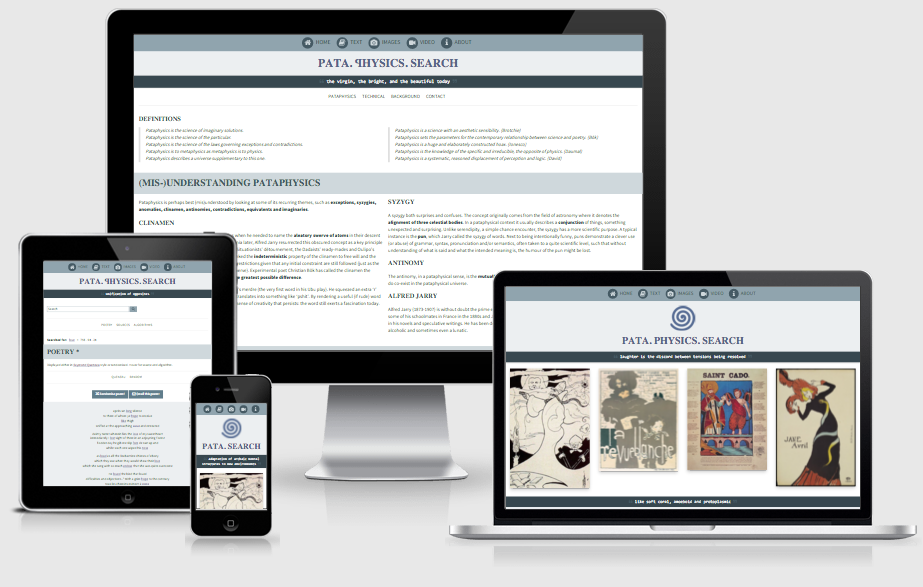
\includegraphics[width=\linewidth]{images/proto3screen}
\caption[Responsive design of \url{pata.physics.wtf}]{Responsive design of \url{pata.physics.wtf}}
\label{img:proto3screen}
\end{figure}

The text results page has three different result styles, with `Poetry --- Queneau' being the default.

\begin{description}[leftmargin=2.8cm]
  \item [Poetry] Displayed in sonnet style (two quatrains and two tercets) if possible, although no rhyming pattern is used\footnote{This is addressed in chapter~\ref{s:textfuture}.}.
    \begin{itemize}
      \item Queneau --- Each line can be changed manually.
      \item Random --- The whole poem can be randomised.
    \end{itemize}
  \item [Sources] Ordered by source text.
  \item [Algorithms] Ordered by algorithm.
\end{description}

The image and video results pages work the same way. They both have two display options, with the `Spiral' option being the default. The spirals are modelled on the idea of golden spirals (more precisely an approximation in the form of a Fibonacci spiral).

\begin{description}[leftmargin=1.8cm]
  \item [Spiral] Displayed as square images/videos in a spiral.
  \item [List] Displayed as a simple list.
\end{description}

The overal visual design is shown in image~\ref{img:proto3screen}\sidepar{\faicon{picture-o}~\ref{img:proto3screen}}.


\subsection{Poetry}
\label{s:poetry}

Source~\ref{code:qpoems}\sidepar{\faicon{code}~\ref{code:qpoems}} shows the segment of \ac{HTML}/Jinja code that renders the Queneau poetry. The code renders the 4 stanzas of the poem. This is done using two nested Jinja \py{for} loops (line 2 and line 10). Line 2 loops through the (ideally) 14 lines of the poem. \py{lol} can be considered a masterlist of all sublists for each poem line.

Functionality for sending the currently showing poem per email is added via a button which calls a JavaScript function \py{onclick="return getContent(this)"} which then retrieves the content of each line in the poem and sends it to the body of the email. 

\py{all_sens} is the pool of all sentences. It is structured as \py{[(title, (pre, word, post), algorithm), ...]}. \py{lol} is a list subdivided into partitions for each line of the sonnet. Let's say there are 350 sentences overall in \py{all_sens}. To divide them equally among the 14 lines of a sonnet, we need to create \py{lol} with 14 equal parts of 25 sentences: \py{[all_sens[0-24], all_sens[25-49], ...,  all_sens[325-349]]}.

% \begin{minted}{text}
%   # all_sens list:
%     [(title, (pre, word, post), algorithm), ...]
%   # lol list:
%     [all_sens[0], all_sens[1], ... all_sens[x]]
%     # where x is the number of possible sentences minus 1 per line in a poem
% \end{minted}

\begin{listing}[!htbp] % (here, top, bottom, page)
  \begin{minted}{html+jinja}
<div>
  
    
    
    
    
    <div id=`poems'>
      <div id=`{{wid}}' class=`wn'>
        <div id=`{{lid}}' class=`lyr'>
          <span title=`{{ sens[0] }}, {{ sens[2] }}'>{{ sens[1][0] }} <form class=`inform' action=`../textresults' method=`post'><input class=`inlink' type=`submit' name=`query' value=`{{ sens[1][1] }}' onclick=`loading();'></input></form> {{ sens[1][2] }}</span>
        </div>
      </div>
      <div id=`{{sid}}' class=`scrollLinks'></div>
    </div>
  
</div>
  \end{minted}
\caption[HTML for Queneau style poems]{Simplified \ac{HTML} code for rendering Queneau style poems}
\label{code:qpoems}
\end{listing}

Changing a line of the poem is achieved by clicking on one of the buttons on either side of the poem's line (as shown in image~\ref{img:qpoemtree}\sidepar{\faicon{picture-o}~\ref{img:qpoemtree}}). This will trigger a JavaScript function (based on \autocite{DYNWEB2016}) to automatically scroll to the next sentence. 

\begin{figure}[!htbp] % (here, top, bottom, page)
  \centering
  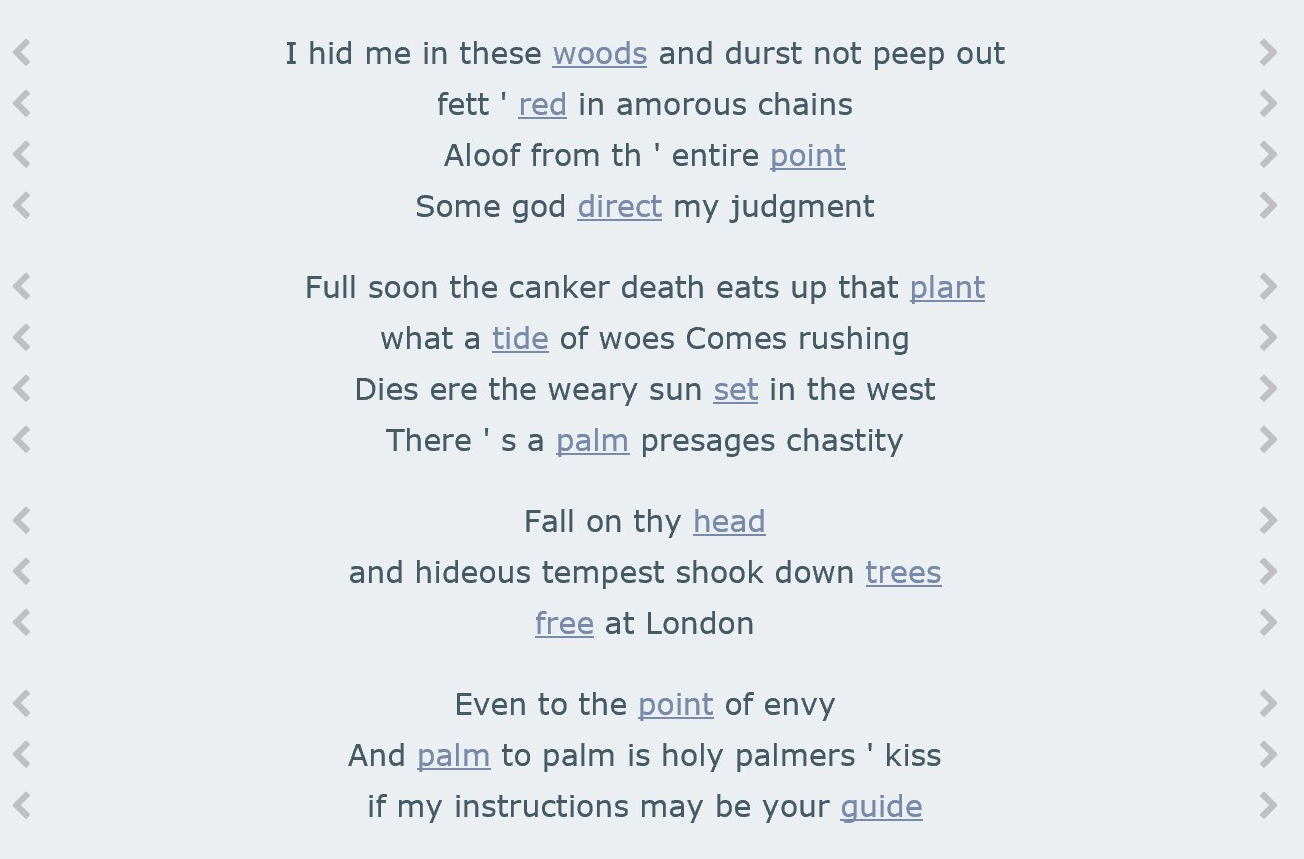
\includegraphics[width=\linewidth]{images/qpoemtree}
\caption[Queneau poem for query `tree']{Example Queneau poem for query `tree'}
\label{img:qpoemtree}
\end{figure}

Non-Queneau poems have a slightly different functionality. It is not possible to change the poem line by line but rather the whole poem can be randomised on demand. This relies on a random number generator in JavaScript. A function \py{shufflePoem()} creates a random variable \py{r} as \py{Math.floor(Math.random() * n)}, which can then be used to generate a new list of 14 lines for the poem randomly selected from the pool of sentences \py{all_sens}.


\subsection{Lists}

The two other ways to display text results are as a list ordered by source or by patalgorithm which works in a similar way to what is described in source~\ref{code:textlists}\sidepar{\faicon{code}~\ref{code:textlists}}. The code is wrapped in an \ac{HTML} unordered list tag \py{<ul>}. A Jinja \py{for} loop generates the individual \py{<li>} tags on line 4.

A \py{sens} in \py{all_sens} is structured as \py{(title, (pre, word, post), algorithm)}. This means that to access the name of the algorithm we need to call the Jinja template \py{{{ sens[2] }}}, to get the first half of the sentence we need \py{{{ sens[1][0] }}}, the middle keyword (i.e. the patadata term) \py{{{ sens[1][1] }}} and the second half of the sentence \py{{{ sens[1][2] }}}.

\begin{listing}[!htbp] % (here, top, bottom, page)
  \begin{minted}{html+jinja}
<ul>
  
    
      <li title=`{{ sens[2] }}'>...{{ sens[1][0] }} <form class=`inform' action=`../textresults' method=`post'><input class=`w3-hide' type=`radio' name=`corpus' value=`{{ corpus }}' checked><input class=`inlink' type=`submit' name=`query' value=`{{ sens[1][1] }}' onclick=`loading();'></input></form> {{ sens[1][2] }}...</li>
    
  
</ul>
  \end{minted}
\caption[HTML for results by source]{Simplified \ac{HTML} code for rendering a list of text results by source}
\label{code:textlists}
\end{listing}

Image~\ref{img:listsourcetree}\sidepar{\faicon{picture-o}~\ref{img:listsourcetree}} shows a shortened example set of results for query `tree' ordered by source, that is, ordered by original file.

\begin{figure}[!htbp] % (here, top, bottom, page)
  \centering
  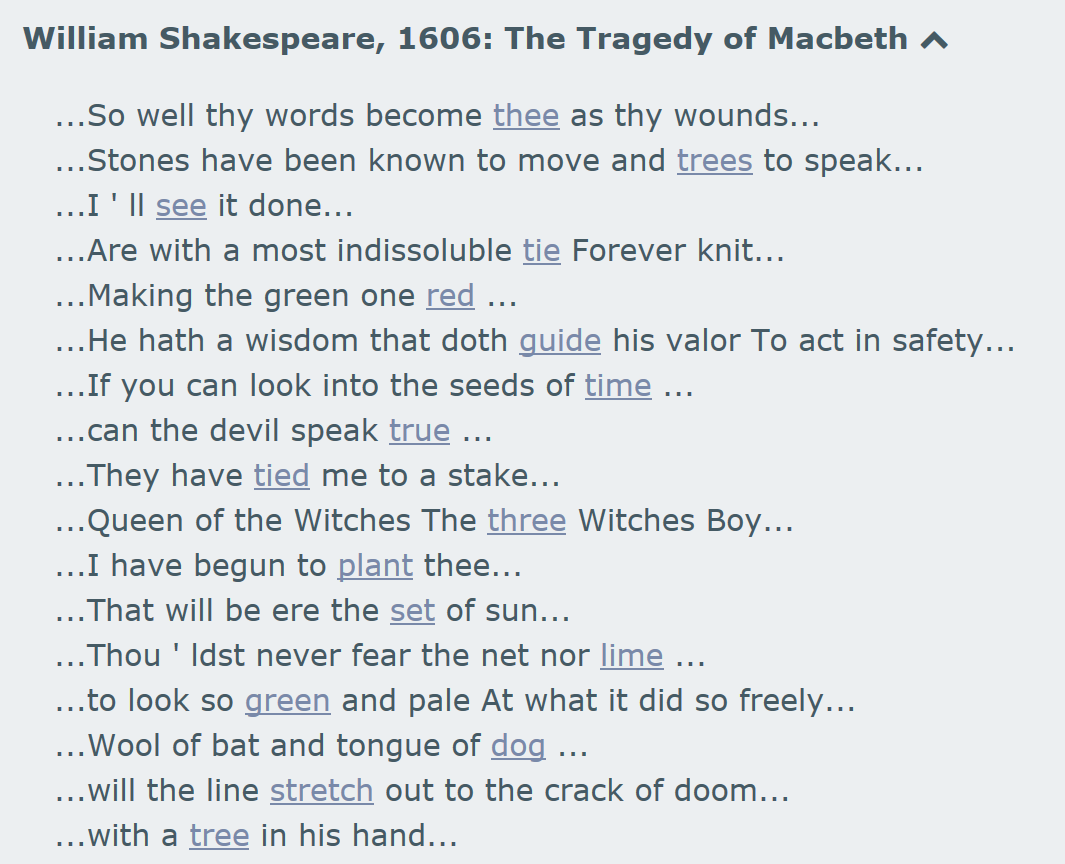
\includegraphics[width=\linewidth]{images/listsourcetree}
\caption[Source result list for query `tree']{Example results for query `tree' ordered by source}
\label{img:listsourcetree}
\end{figure}

Image~\ref{img:listalgotree}\sidepar{\faicon{picture-o}~\ref{img:listalgotree}} shows a shortened example set of results for query `tree' ordered by patalgorithm, that is, ordered by the algorithm which produced the patadata.

\begin{figure}[!htbp] % (here, top, bottom, page)
  \centering
  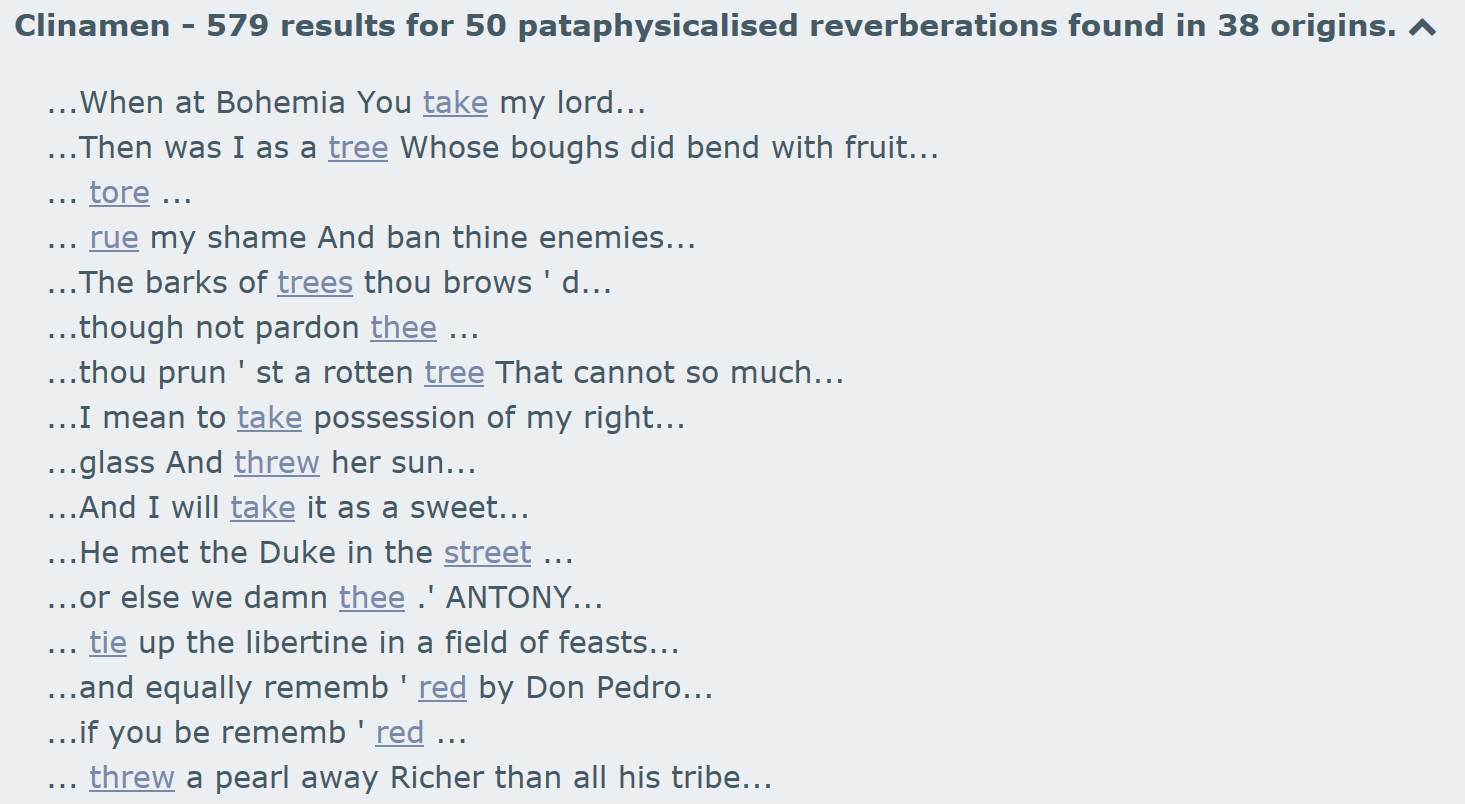
\includegraphics[width=\linewidth]{images/listalgotree}
\caption[Source result list for query `tree']{Example results for query `tree' ordered by patalgorithm}
\label{img:listalgotree}
\end{figure}


\subsection{Spiral}
\label{s:spiral}

The image and video spirals are constructed in complicated nested \ac{HTML} components. The code for generating an image spiral is shown in appendix~\ref{s:imgspiral}\sidepar{§~\ref{s:imgspiral}}. The video spiral is constructed in a similar way but directly in the \ac{HTML} file as opposed to in the JavaScript file. The video spiral is almost identical, the only difference is that only the biggest 5 videos are atually embedded as videos. The smaller 5 videos are shown as still images which link to the relevant YouTube page.

Generally, the idea was taken from the pataphysical \emph{grand gidouille} (see chapter~\ref{ch:pataphysics}\sidepar{§~\ref{ch:pataphysics}}) and represented as a Fibonacci spiral. 

Figure~\ref{img:fibspiral}\sidepar{\faicon{object-group}~\ref{img:fibspiral}} shows a spiral created using the Flickr image search for query `blue mountains' overlaid with a white Fibonacci spiral to highlight the structure.

\begin{figure}[!htbp] % (here, top, bottom, page)
  \centering
  \begin{tikzpicture}
    \node[anchor=south west] at (-10.8,-2.7) {\includegraphics[width=14.7cm, height=9.1cm]{images/bluemountains-flickr}};
    \begin{scope}[rotate=180, xshift=6.6cm, yshift=-4cm, draw=white,ultra thick]
      % Example from http://www.texample.net/tikz/examples/fibonacci-spiral/
      \newcounter{a}
      \newcounter{b}
      \newcounter{temp}
      \setcounter{a}{0}
      \setcounter{b}{1}
      \coordinate (0) at (0,0);
      \foreach \i in {1,...,18}
      {
        \pgfmathsetmacro{\lastpoint}{\i-1}
        \pgfmathsetmacro{\startangle}{mod(\i-1,4) * 90}
        \draw (\lastpoint) arc 
          (\startangle : \startangle + 90 : \value{b}/10.0pt) coordinate (\i);
        \setcounter{temp}{\value{b}}
        \addtocounter{b}{\value{a}}
        \setcounter{a}{\value{temp}}
      }
      \foreach \i in {1,3,...,17}
      {
        \pgfmathsetmacro{\lastpoint}{\i-1}
        \draw (\lastpoint) -| (\i);
      }
      \foreach \i in {2,4,...,16}
      {
        \pgfmathsetmacro{\lastpoint}{\i-1}
        \draw (\lastpoint) |- (\i);
      }
      \draw (17) -- (17 |- 18);
    \end{scope}
  \end{tikzpicture}
  \caption[Fibonacci image spiral]{Fibonacci spiral overlaid onto an image results for query `blue mountains' using Flickr}
  \label{img:fibspiral}
\end{figure}


\section{Prototypes}
\label{s:prototypes}

The final website \url{pata.physics.wtf} went through several iterations of development since it was first conceived in 2012. This included 3 major technical updates since the first prototype and 2 new visual re-designs.

Table~\ref{tab:versions}\sidepar{\faicon{table}~\ref{tab:versions}} shows the main differences and similarities between the versions. 

\begin{table}[!htbp]
  \centering
  \footnotesize
  \caption[Comparison of different versions of \url{pata.physics.wtf}]{Comparison of different versions of \url{pata.physics.wtf}}
  \label{tab:versions}
  \begin{tabu}{X[l]X[l]X[l,1.2]X[l,1.5]X[l,2]}
  \toprule
  & \textbf{Version 1} & \textbf{Version 2} & \textbf{Version 3} & \textbf{Version 4} \\ 
  \midrule
  \textbf{Language(s)} & Python, Django & Python, Flask & Python, Flask & Python, Flask, JavaScript \\
  \textbf{Server} & Django, Heroku & Flask, Mnemosyne & Flask, Gunicorn, Mnemosyne & Flask, Gunicorn, OVH \\
  \textbf{Features} & Text & Text, Image, Video & Text, Image, Video & Text, Image, Video \\
  \textbf{Corpus} & Faustroll text & Faustroll text & Faustroll's library & Faustroll's library and Shakespeare \\
  \textbf{API's} & WordNet & WordNet, Flickr, Bing, YouTube, Microsoft Translator & WordNet, Bing, YouTube, Microsoft Translator & WordNet, Flickr, Getty, Bing, YouTube, Microsoft Translator \\
  \textbf{Design} & Algorithms & Algorithms, Spiral & Algorithms, Source, Poetry, Spiral, List & Algorithms, Source, Poetry, Spiral, List \\ 
  \textbf{Responsive} & No & Yes & Yes & Yes \\ 
  \bottomrule
  \end{tabu}
\end{table}

Images~\ref{img:proto1screen}, \ref{img:proto2screen} and \ref{img:proto3screen} show the 3 main visual designs.

\begin{figure}[!htbp] % (here, top, bottom, page)
  \centering
  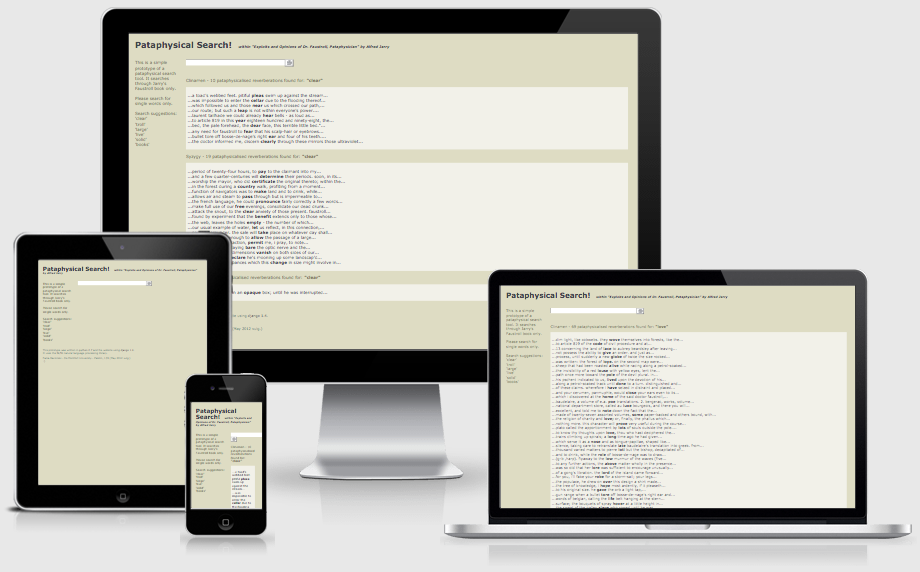
\includegraphics[width=\linewidth]{images/proto1screen}
\caption[First version of \url{pata.physics.wtf}]{First version of \url{pata.physics.wtf}}
\label{img:proto1screen}
\end{figure}

\begin{figure}[!htbp] % (here, top, bottom, page)
  \centering
  
\includegraphics[width=\linewidth]{images/proto2screen}
\caption[Second major version of \url{pata.physics.wtf}]{Second major version of \url{pata.physics.wtf}}
\label{img:proto2screen}
\end{figure}

The latest version, which is now live at \url{pata.physics.wtf}, introduced major changes to the initial setup stage of the system and a lot of the code was refactored and improved. As of the date of writing this, there were over 360 commits in the git repository since 2012. See appendix~\ref{s:gitweb}\sidepar{§~\ref{s:gitweb}}.


\stopcontents[chapters]
